\documentclass[12pt]{article}

% Basic stuff
\usepackage{fullpage}
\usepackage{graphicx}
\usepackage[parfill]{parskip}
\usepackage[utf8]{inputenc}

% Skip one line between paragraphs
\parskip1em
 
% Standard things to include for math   
\usepackage{amsmath,amssymb,amsfonts,amsthm}

% Other stuff
\usepackage{hyperref}
\usepackage{datetime} \usdate
\usepackage{enumitem}
\usepackage{changepage}
\usepackage{tcolorbox}
\usepackage{tikz}
\usepackage{xcolor}
\hypersetup{
    colorlinks,
    linkcolor={red!50!black},
    citecolor={blue!50!black},
    urlcolor={blue!80!black}
}


% Some of Ebrahim's definitions
\newcommand{\note}[1]{[#1]}
\newcommand{\done}{\\\hspace*{0pt}\hfill$\blacksquare$}
\def\N{\mathbb{N}}
\def\R{\mathbb{R}}
\def\Q{\mathbb{Q}}
\def\Z{\mathbb{Z}}
\def\e{\varepsilon}
\def\d{\delta}
\newcommand{\seq}[1]{\left(#1\right)_{n\in\N}}
\renewcommand{\emptyset}{\{\hspace{-2pt}\}}
\newcommand{\powerset}[1]{\mathcal{P}(#1)}
\newcommand{\dom}[1]{\operatorname{dom}(#1)}
\newcommand{\ran}[1]{\operatorname{ran}(#1)}
\newcommand{\rev}[1]{(#1)^{\dashv}}
\newcommand{\injrightarrow}{\xrightarrow{\text{inj}}}
\newcommand{\surjrightarrow}{\xrightarrow{\text{surj}}}
\newcommand{\bijrightarrow}{\xrightarrow{\text{bij}}}
\newcommand{\AND}{\wedge}
\newcommand{\OR}{\vee}
\newcommand{\ARR}{\Rightarrow}
\newcommand{\DARR}{\Leftrightarrow}

\def\bbel{
\,
\raisebox{-2pt}{
\includegraphics[scale=0.8]{bbel.pdf}}
\,
}

\newcommand{\ALL}[2]{\left(\,\forall{#1}\,\bbel\,#2\,\right)}
\newcommand{\EXIST}[2]{\left(\,\exists{#1}\,\bbel\,#2\,\right)}
\newcommand{\COLL}[2]{\left\{\, {#1} \,\bbel\, {#2} \, \right\}}
\newcommand{\settext}[2]{\COLL{#1}{\text{#2}}}

%\newcommand{\SUBST}[3]{{#1}\left[{#2}\mapsto{#3}\right]}
%\newcommand{\SUBST}[3]{{#1}_{{#2}\mapsto{#3}}}
\newcommand{\SUBST}[3]{{#1}_{[{#2}\rightarrow{#3}]}}
%\newcommand{\SUBST}[3]{{#1}\,\text{replacing}\,{#2}\,\text{by}\,{#3}}
%\newcommand{\SUBST}[3]{{#1}\ \text{replacing}\ {#2}\ \text{by}\ {#3}}

%\newcounter{exercise}[subsubsection]
\newcounter{exercise}
\newcounter{rule}
\newcounter{theorem}
%\def\theexercise{\thesubsubsection.\arabic{exercise}}

\def\putExerciseHeading{\refstepcounter{exercise} \textbf{Exercise \theexercise}}
\def\putRuleNumber{\refstepcounter{rule}\therule}
\def\putThmNumber{\refstepcounter{theorem}\thetheorem}

\newcommand{\ex}[1]{ \putExerciseHeading: \begin{adjustwidth}{2em}{}#1\end{adjustwidth}}
\newcommand{\indented}[1]{\begin{adjustwidth}{1em}{}#1\end{adjustwidth}}


\def\thmcolonspace{\hspace{1em}}
\def\proofnewline{\\[0.75em]} % Separates theorem box from proof, no new paragraph expected.
\def\proofsep{\\[-0.5em]} % Separates different proofs (e.g. to diff parts of same theorem). No new paragraph expected.
\renewcommand\qedsymbol{$\blacksquare$}
\def\done{\qed\\[0em]} % QED with newline so that QED symbol is flushed to the right. IDK why newline is needed for this to happen.
\newcommand{\thmbox}[1]{\fbox{\parbox{\textwidth}{{#1}}}}
\newcommand{\THMMOCK}[2]{\thmbox{\textbf{Theorem:} \thmcolonspace #1} \proofnewline \textit{Proof:} #2\done}
\newcommand{\THMP}[2]{\thmbox{\textbf{Theorem \putThmNumber:} \thmcolonspace #1} \proofnewline\textit{Proof:} #2\done}
\newcommand{\THMNP}[3]{\thmbox{\textbf{Theorem \putThmNumber\ (#1):} \thmcolonspace #2} \proofnewline\textit{Proof:} #3\done}
\newcommand{\THM}[1]{\thmbox{\textbf{Theorem \putThmNumber:} \thmcolonspace #1}}
\newcommand{\THMN}[2]{\thmbox{\textbf{Theorem \putThmNumber\ (#1):} \thmcolonspace #2}}
\newcommand{\AXIOM}[1]{\thmbox{\textbf{Axiom \putThmNumber:} \thmcolonspace #1}}
\newcommand{\AXIOMN}[2]{\thmbox{\textbf{Axiom \putThmNumber\ (#1):} \thmcolonspace #2}}
\newcommand{\DEFN}[2]{\thmbox{\textbf{Definition \putThmNumber\ (#1):} \thmcolonspace #2}}


\newcommand{\RULE}[2]{\begin{tcolorbox}[title=Rule \putRuleNumber: #1,colbacktitle=white,coltitle=black,colback=white]#2\end{tcolorbox}}
\newcommand{\DRULE}[2]{\begin{tcolorbox}[title=Derived Rule \putRuleNumber: #1,colbacktitle=white,coltitle=black,colback=white]#2\end{tcolorbox}} % IDK if derived rules will be different
\newcommand{\DRULEPF}[3]{\begin{tcolorbox}[title=Derived Rule \putRuleNumber: #1,colbacktitle=white,coltitle=black,colback=white] {#2} \tcblower \textbf{Proof:} {#3} \end{tcolorbox}}
\newcommand{\DRULEPZ}[2]{\begin{tcolorbox}[title=Derived Rule \putRuleNumber: #1,colbacktitle=white,coltitle=black,colback=white] {#2} \tcblower \textbf{Proof:} 
                         \putExerciseHeading. \end{tcolorbox}}

\def\pA{\Phi}
\def\pB{\Psi}
\def\pC{\Omega}
\def\pD{\Sigma}
\def\pE{\Gamma}
\def\pF{\Delta}




\begin{document}

\begin{center} {\Large \scshape Mathematical Proofs and Mathematical Writing}
\end{center}
(compiled on \today\ at\ \currenttime)
\hfill

\tableofcontents

\section{Introduction}

%\note{what to put here:
%this course is about both set theory and writing.
%set theory is axiomatic. describe what i mean by that, why we would do that, and the historical relevance of it.
%why rigor anyway?
%logic can also be done this way, but we will not.
%we will follow a more intuitive and informal writing-focused approach for logic,
%saving our rigor-enegery for set theory.
%perhaps include a discussion levels of rigor and formality, with one level relegating the rigor to other levels.
%mention the importance of writing and the roughness of this transition for many people.
%mention the value of forgetting what you knew before, but not really forgetting it all.}
%an illustration containing two towers, one of the math t hey built up till now, and one new tower starting here of the math they are now building

\note{Write the general intro later, maybe last.}



\section{Mathematical Language}
\label{sec:logic}

This section will develop mathematical logic and show you how logical arguments factor into writing.
We do not yet have anything to argue \emph{about}, so our ``proofs'' will be about nothing in particular.
Section \ref{sec:sets} will later give some mathematical objects to talk about, and we will then put
content into the empty skeleton arguments of this section.

\subsection{Parts of Speech}
\label{sec:parts_of_speech}

In a language, a \emph{part of speech} is a collection of words that share grammatical properties.
For example here are some common English parts of speech: pronouns, nouns, verbs, adjectives, and adverbs.
Different languages can have different parts of speech that are useful for describing their grammar.
To build up the grammar of a language, one can specify how parts of speech fit together to form larger
\emph{constituents}, such as noun phrases and clauses. One can further describe how
constituents fit together to form even more complex constituents, eventually grammatical sentences.

Mathematics is a language, and so it makes sense to build up its grammar (its \emph{syntax}) using this same strategy.
Instead of pronouns, nouns, verbs, noun phrases, sentences, and so on, there are just four constitutuents in
mathematics. Two are basic parts of speech and two are more complex constituents:
\begin{itemize}
\item \emph{Variables} are a basic part of speech.
\item \emph{Constants} are a basic part of speech.
\item \emph{Terms} can be built out of variables, constants, other terms, and propositions.
\item \emph{Propositions} can be built out of variables, constants, terms, and other propositions.
\end{itemize}

Let's go through each of these in detail.

\def\sp{\hspace{1em}}
\paragraph{Variables}
Variables serve as placeholders, waiting to be replaced by other symbols.
They are most like pronouns in English.
For example the pronoun ``it'' is a placeholder referring to something in a discussion, but what it refers to depends on the context of the discussion.
Variables are like that.
Here are some variables:
\begin{center}
$a$ \sp $b$ \sp $A$ \sp $f$ \sp $q$ \sp $x$\sp $\alpha$\sp $\beta$
\end{center}
Variables are copies of letters coming from an alphabet (usually Latin or Greek) and written in ink/chalk/pixels.



\def\sp{\hspace{1em}}
\paragraph{Constants}
Constants are used as fixed names for specific mathematical objects.
They are most like \emph{proper} nouns in English.
Here are some constants:
\begin{center}
$0$ \sp $1$ \sp $2$ \sp $3$ \sp $4$ \sp $5$ \sp $6$ \sp $7$ \sp $8$ \sp $9$ \sp $\N$ \sp $\R$ \sp $\emptyset$
\end{center}
The difference between constants and variables is that constants are not meant to be substituted for.
The constant ``$2$'' refers to a specific thing, rather than being a placeholder for something.


Note that we are mainly talking about elements of \emph{language}, and not about what those elements \emph{refer} to.
Germany is not a noun, it's a country. ``Germany'' is, however, a noun.
Similarly, we can say that $2$ is not a constant, but rather ``$2$'' is.
And $x$ is not a variable, but rather ``$x$'' is.
Quotation marks help us make the distinction between a symbol and what the symbol refers to
(though I will often be lazy and drop the quotation marks).




\def\sp{\hspace{1em}}
\paragraph{Terms}
Terms are strings of marks (expressions) that refer to \emph{mathematical objects}.
Since variables and constants refer to mathematical objects, they are special cases of terms.
But you can also have more complicated terms that are built out of simpler ones.
Terms are most like \emph{noun phrases} in English.
For example the phrase ``the cup that you drank from'' is a noun phrase;
it doesn't make any assertion but rather it just refers to a \emph{thing}.
Here are some terms:
\begin{itemize}[label=\sp]
\item $x$
\item $7$
\item $\{2,3,a,7\}$
\item $f(x)$
\item $\{(z,w)\} \circ g$
\item $S\times Q$
\item the square of the seventh prime number
\item a triangle
\item twelve dimensional euclidean space
\item the collection of even integers
\item $\settext{n}{$n\in\Z$ and $n$ is even}$
\item $\settext{n}{$(n\in\Z)\AND (\exists k\,|\,(k\in\Z)\AND(2k=n))$}$
\end{itemize}
The last three terms actually refer to the same mathematical object; this will soon become clear
when we get into \emph{how} the symbols refer to objects (semantics). For now we are only looking at
\emph{which} strings of symbols \emph{can} refer to objects (syntax).
You can see that some terms are more ``symbolic,'' while others are more ``Englishy.''
The formal language of mathematics is purely symbolic,
but we almost never use the language in its purest form.
Typically, we communicate by some combination of English and mathematics.


\def\sp{\hspace{1em}}
\paragraph{Propositions}
Propositions are strings of marks (expressions) that \emph{make assertions}.
They are most like \emph{sentences} in English (declarative sentences).
Propositions can be true or false. 
Here are some propositions:
\begin{itemize}[label=\sp]
\item $x\in S$.
\item $5\notin x$.
\item $0=2$.
\item $(x\neq y) \AND (x\neq z) \AND (y\neq z)$.
\item $x$, $y$, and $z$ are distinct.
\item Either $A\subseteq P$ or $x\in S$, but not both.
\item $f:X\rightarrow Y$.
\item If $x\in S$, then we either have $x\notin W$ or we have $x\in\Z$.
\item $\neg(X\times Y \subseteq Z)$.
\item Every integer is even.
\item $\ALL{n}{(n\in\Z)\ARR \EXIST{k}{(k\in\Z)\AND(2k=n)}}$.
\end{itemize}
The last two propositions are actually saying the same thing, as we will see when we get into semantics.
Again, you can see that some propositions are more ``symbolic,'' while others are more ``Englishy.''
Typically, we make mathematical assertions by using some combination of English and mathematics.
The English that we use is a crude, but human-friendly, stand-in for formal mathematical statements.



\ex{
Determine whether each of the following is a term or a proposition.
\begin{enumerate}
\item $n$
\item $1+1=0$
\item $n$ is an odd integer
\item an odd integer
\item $f$ is a function with domain $S$
\item $1+(2+3)$
\item the empty set
\item the sum of two vectors is another vector
\item the zero vector
\item the evenness of $2$ % this one is a trick, it's neither unless you are doing metamathematics
\end{enumerate}
}

\subsection{Theorems and Proofs}

Mathematics is ultimately about propositions.
Propositions \emph{say} things, sometimes true things and sometimes false things.
We want to know: Which propositions are true? What does ``true'' even mean?
We will not exactly define ``true,'' but we will define ``provable,''
and provability will be our notion of truth.

The rules of logic allow us to make deductions and \emph{prove} new propositions
from already proven propositions.
Those already proven propositions themselves had to be proven via a sequence of logical deductions
that was applied to other previously proven propositions.
And so on...
but where does it all start?

\paragraph{Axioms}
Some propositions are declared to be \emph{axioms},
which makes them serve as starting points in our mathematical system.
The next paragraph will clarify this.

\paragraph{Proofs}
A \emph{proof} is a sequence of propositions such that each proposition is either
(1) an axiom, 
(2) an already proven proposition,
or, (3) the result of applying the rules of logic to \emph{previous} propositions in the sequence.
A proposition that appears in a proof is said to be \emph{proven}.


\paragraph{Theorems}
A \emph{theorem} is a proposition which is asserted to have a proof.

\subsubsection{Example of a Formal Proof}


\def\ES{\settext{x}{$x\neq x$}}

Below is an example of a proof of the proposition ``$(\forall x\,|\,x\notin\ES)$''.
\begin{adjustwidth}{1cm}{}
$(x\in\ES)\Longrightarrow (x\neq x)$\\ 
$(x=x)\Longrightarrow (x\notin \ES)$\\
$x=x$\\
$x\notin\ES$\\
$(\forall x\,|\,x\notin\ES)$
\end{adjustwidth}
Here I don't want you to worry about interpreting what the propositions are trying to \emph{say};
I just want to demonstrate how a theorem arises as a result of applying the rules of logic
to various axioms. What you see above is a sequence of five propositions, ending with the
one I claimed to be proving, namely ``$(\forall x\,|\,x\notin\ES)$''.
To really be convinced that we are looking at a proof, we would need a \emph{justification}
for each of the five propositions-- for each proposition we need to either point out that it is
an axiom, or we need to verify that it follows logically from the previous propositions.
In this example, two of the propositions are axioms, and the other three are logical deductions;
here is a schematic depiction of these relationships:
\begin{center}
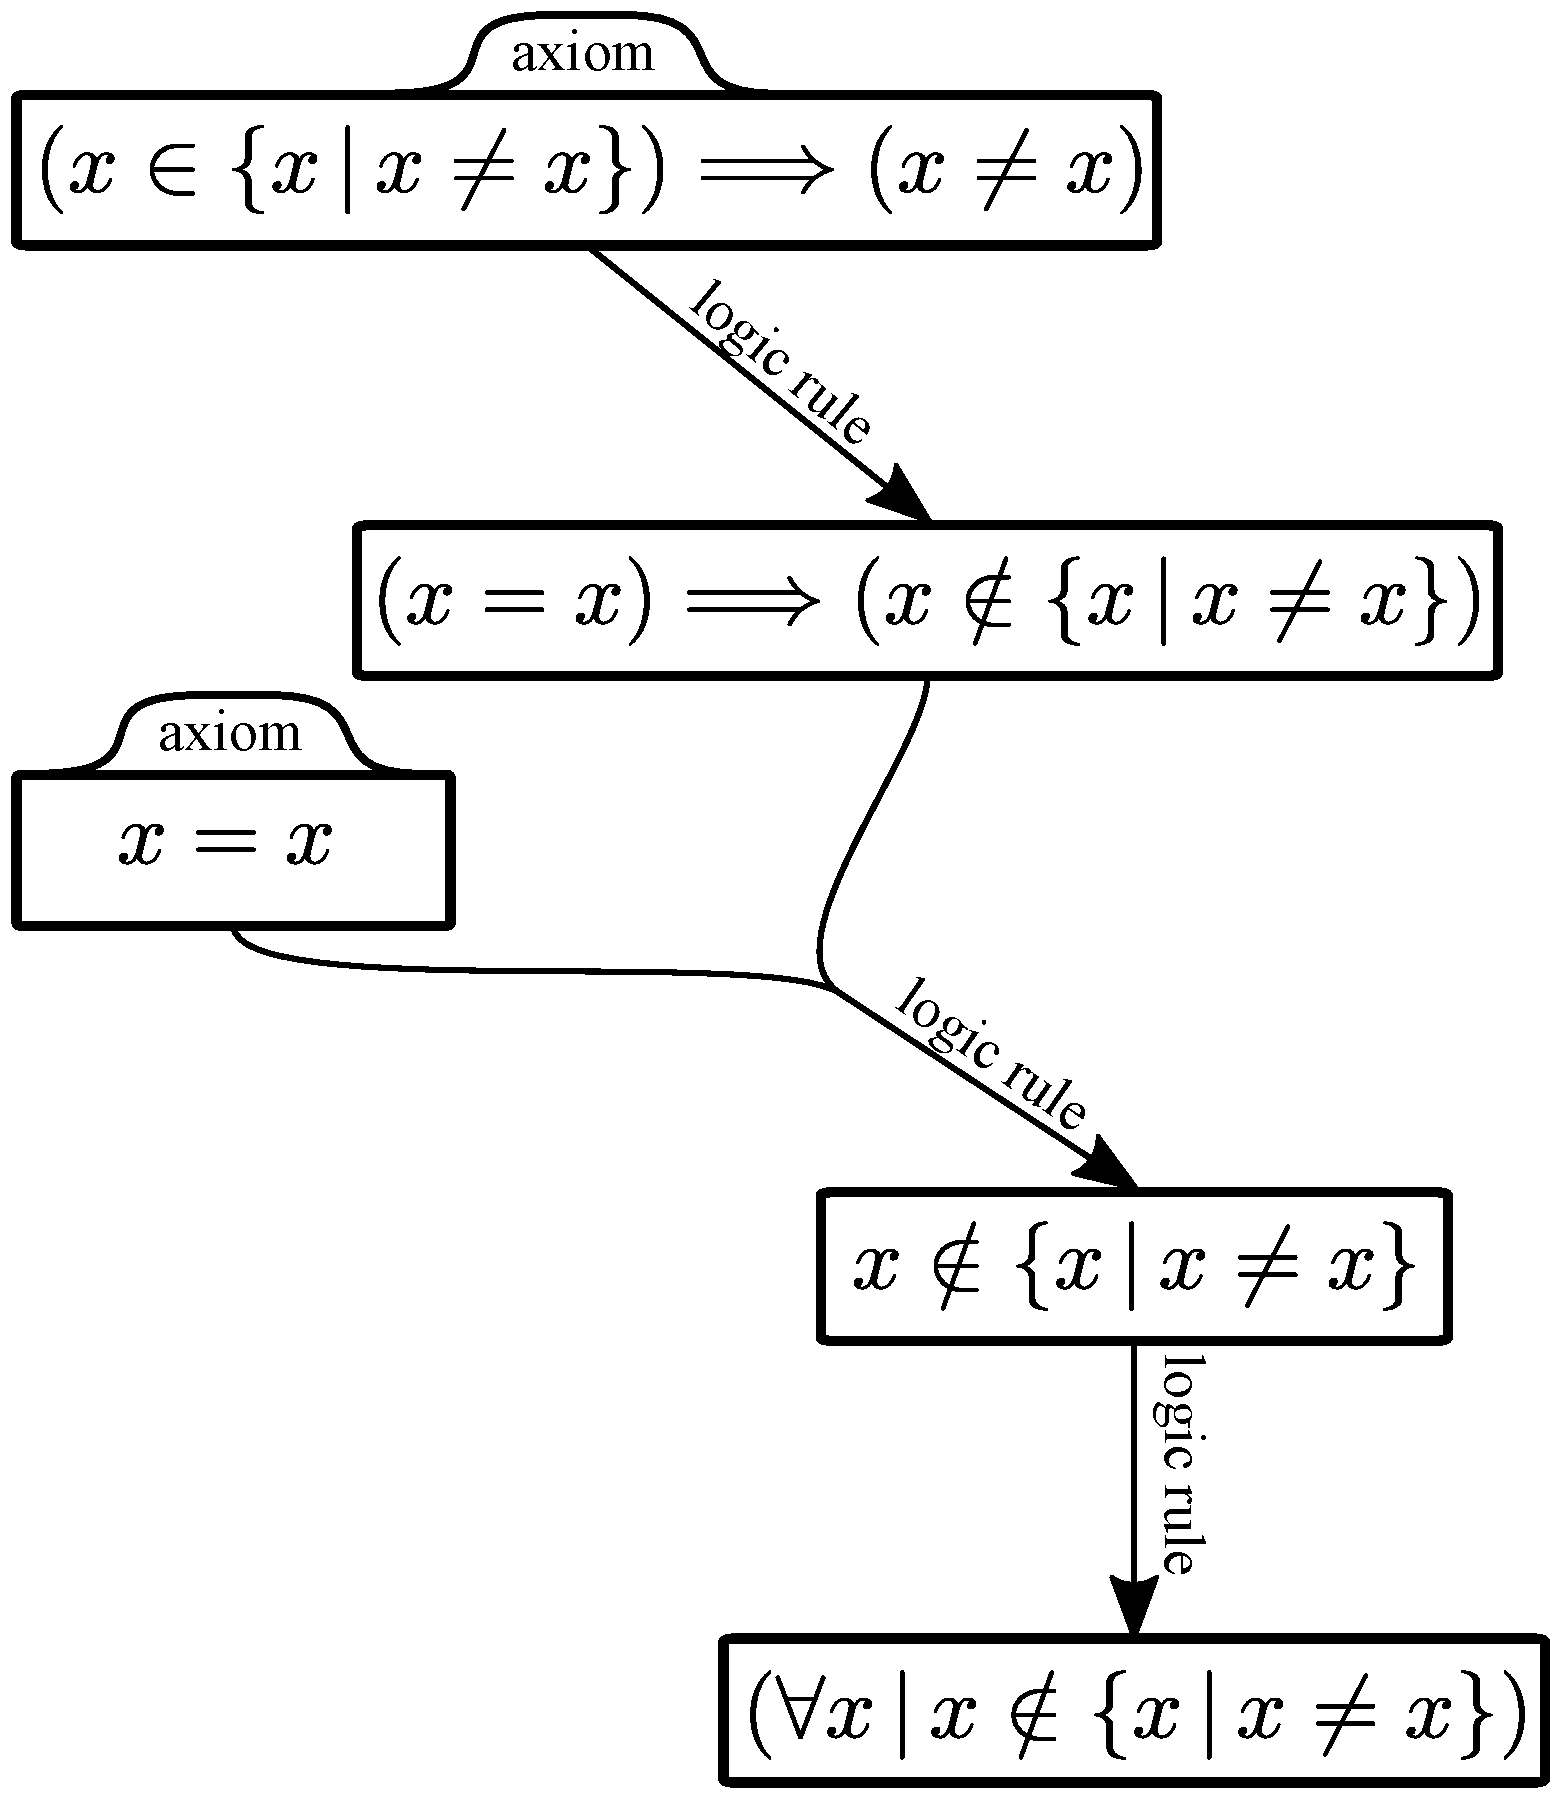
\includegraphics[scale=0.25]{proofFlow.pdf}
\end{center}
Again, don't worry yet about understanding why this works.
What I want you to take away from this is the general structure:
we have axioms serving as starting propositions, and we use logic to ``flow'' out from
the starting points and prove other propositions.

Given a bunch of axioms to start with, what theorems can we deduce?
To answer this question is to do math.

\paragraph{Remark about Axioms}
Axioms often serve to \emph{give meaning} to symbols.
For example, the axiom $x=x$ (along with some other axioms related to equality)
gives meaning to the symbol ``$=$''.
Without the axiom, we would still be able to form propositions like $a=b$ but we would never be able to
prove anything about them.
Suppose you ``disagree'' with the axiom $x=x$ and instead use some other propositions related to ``$=$'' as axioms.
That's perfectly fine-- you would just be giving a different meaning to the symbol ``$=$'' and it would serve a different purpose in your language.

\paragraph{Math is for Humans}
The five-line proof given above is a \emph{formal proof}-- it is written in pure mathematical language
with absolutely no English.
This is great if you want absolute rigor, but
it is not friendly to read if you are not a computer.
The main purpose of a mathematical proof is for it to convince a human that a theorem is true.
But formal proofs make for really inefficient communication between humans.
Thus we are faced with a trade-off: 
we can sacrifice some rigor to gain efficiency of communication.

\emph{Informal proofs} use a mixture of English and mathematics to make arguments.
For an example, look ahead a few paragraphs for an informal version of the five-line proof above.

We need to find a good balance between rigor and efficient communication.
Finding that balance is one of the great challenges when you first learn how to write proofs.
If we sacrifice too much rigor in an argument, then we can lose confidence in its correctness.
Or worse, we can start to prove false things!
When developing a new mathematical theory, it's generally good to err on the side of being more rigorous.
Then, as the theory develops and common patterns of arguments become routine,
one can slowly relax the rigor in favor of efficiency.

Now you can see what this course is all about.
While it is partly giving you some specific mathematical content like set theory,
this course is mainly about how to communicate proofs in that balanced way-- rigorous, yet informal and efficient.

Here is an informal version of the five-line proof from above.

\THMMOCK{The set $\ES$ has no elements.}{
If $\ES$ did have an element, say $x$, then we would have $x\neq x$.
But in fact it is an axiom that $x=x$. Thus $\ES$ cannot have any elements.
}

The arguments are essentially the same ones that appeared in the five-line formal proof.
But, compared to the formal proof, it's much easier to process the arguments
in the informal proof
(though I'm still not expecting you to do so just yet).

\newpage 
\def\s{0.25}
\newcommand{\rb}[1]{\raisebox{-0.2em}{#1}}
\ex{
In this exercise we will work with a made-up deductive language which works as follows:
\begin{itemize}
\item Propositions are the only part of speech. The propositions are $3\times 3$ grids in which each square is either blank or contains a dot. Here are three random example propositions:
\begin{center}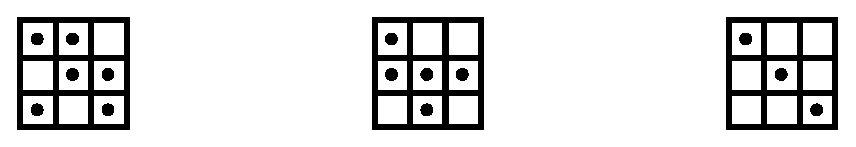
\includegraphics[scale=\s]{gridgame1.pdf}\end{center}
\item There are two logical rules in this language.
The first rule is that if a particular proposition holds, then
its clockwise rotation by ninety degrees follows. So if 
\rb{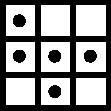
\includegraphics[scale=\s]{gridgame2.pdf}}
holds, then you can deduce that
\rb{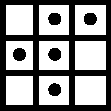
\includegraphics[scale=\s]{gridgame3.pdf}}.
The second rule is that if two propositions $\pA$ and $\pB$ hold, then you can deduce a third proposition
which contains a dot in any square that has a dot in either $\pA$ or $\pB$, but not both.
So for example if you have the two propositions
\rb{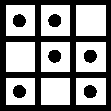
\includegraphics[scale=\s]{gridgame6.pdf}}
and
\rb{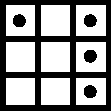
\includegraphics[scale=\s]{gridgame7.pdf}},
then you can deduce from them that
\rb{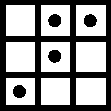
\includegraphics[scale=\s]{gridgame5.pdf}}.
\item There are only two axioms in this language, and they are as follows:
\begin{center}
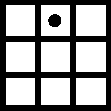
\includegraphics[scale=\s]{gridgame8.pdf}
\hspace{2em}
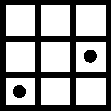
\includegraphics[scale=\s]{gridgame9.pdf}
\end{center}
\end{itemize}
As a demonstration of this deductive language, here is a proof that 
\rb{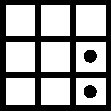
\includegraphics[scale=\s]{gridgame11.pdf}}\ :
\begin{center}
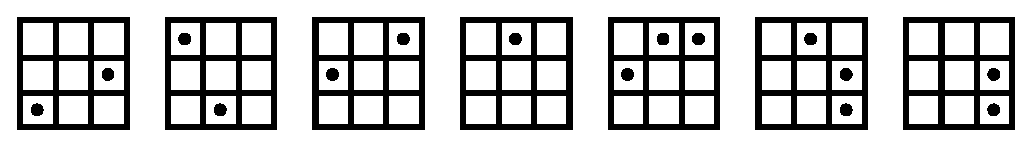
\includegraphics[scale=\s]{gridgame10.pdf}
\end{center}
Can you see how this proof is correct?
These annotations may help:
\begin{center}
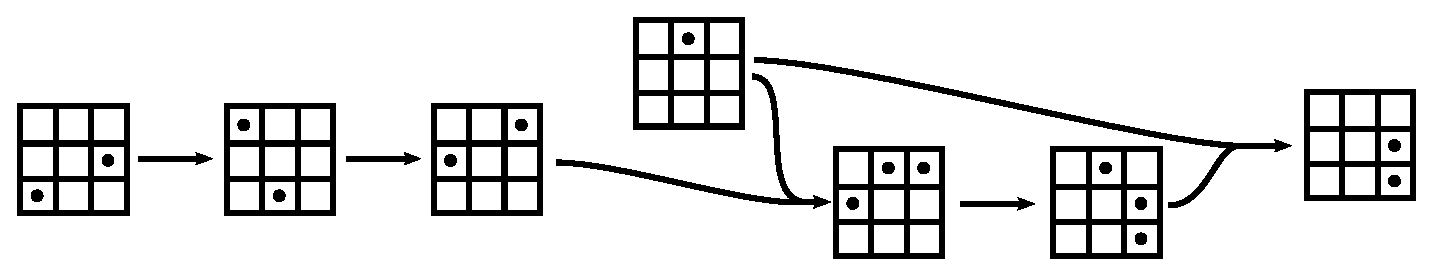
\includegraphics[scale=\s]{gridgame12.pdf}
\end{center}
Now...
\begin{enumerate}
\item
How many propositions are there in this language?
How many propositions do you think there are in mathematics?
How many sentences are there in English?
\item
Give a completely formal proof that 
\rb{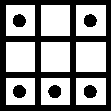
\includegraphics[scale=\s]{gridgame0.pdf}}.
To help out your reader, annotate the proof with arrows like in the example above.
\item (Open-ended) Can you think of a way to write an \emph{informal} version of your proof?
It would be an English description of your proof that does not explain every detail but still captures the essence of your formal proof.
%One way to think of an informal proof is: it somehow gives the reader \emph{instructions} for how to come up with the formal proof.
\item (Irrelevant but fun) Can you figure out how many propositions in this language are provable and how many are not?
\end{enumerate}
}



\subsection{Logic and Writing Mathematical Arguments}

The rest of this course will introduce logic and set theory, starting with logic in this section.
Our goal with logic is not only to understand the rules of deduction,
but also to gain the ability to \emph{write} paragraph-style deductive arguments-- informal proofs.

Logic is all about manipulating \emph{propositions}, so you will not see many \emph{terms} showing up in this section.
In fact, we will find ourselves having to discuss proofs while having nothing in particular to prove anything about.
Mathematical propositions are supposed to say things about mathematical objects;
without any mathematical objects in hand, we cannot form any actual mathematical propositions.
We will proceed with the discussion anyway, using two strategies:

First, we will use capital Greek letters as placeholders for mathematical propositions. Examples include
$$
\pA,
\pB,
\pC,
\pD,
\pE,
\pF.
$$
When you see these capital Greek letters, remember that they are \emph{not variables},
at least not in the sense of mathematical variables. They are not to be replaced by mathematical \emph{objects}.
Rather, they are meant to be replaced by \emph{propositions}.
When they appear in English sentences, they will take the grammatical role of independent clauses.
So, for example, we accept the following as grammatically correct English sentences:
\begin{adjustwidth}{2em}{}
I believe that $\pA$.\\
They thought that $\pA$, but in fact $\pB$.\\
$\pA$.
\end{adjustwidth}

Our second strategy
%for discussing logic without the ability to form mathematical propositions 
is to apply the rules of logic to English sentences.
Even though $\pA$, $\pB$, etc. are supposed to stand for \emph{mathematical} propositions,
we will allow ourselves to replace them by declarative sentences in \emph{English}.
For example, replacing $\pA$ by ``Jim stole the car'' and $\pB$ by ``Jim is an upstanding guy'' in the above examples, we get the sentences
\begin{adjustwidth}{2em}{}
I believe that Jim stole the car.\\
They thought that Jim stole the car, but in fact Jim is an upstanding guy.\\
Jim stole the car.
\end{adjustwidth}
Later when we reach section
\ref{sec:sets}, we will start to work with actual mathematical propositions.

Section \ref{sec:logic_summary}
contains a reference table summarizing the logical constructions that are about to show up;
you can look there to get a sense for what is to come.

\ex{
Which of the following are grammatically correct? Hint: replace Greek letters with English sentences and see what makes sense.
\begin{enumerate}
\item She said that $\pC$, and I think she's onto something.
\item Take that, you accursed $\pA$!
\item Why don't we just $\pB$?
\item To $\pA$, or not to $\pA$, that is the question.
\item Whether $\pC$ or $\pD$, it will always be the case that $\pA$.
\item $\pD$ and $\pF$, but not $\pB$.
\item Despite all the $\pE$, they still wanted to $\pF$.
\item Whenever $\pC$, it turns out that $\pE$.
\item It is not true that $\pA$.
\end{enumerate}
}



\subsubsection{And, Or, and Not}

\paragraph{Conjunction}
\hypertarget{hl:AND}{Given} propositions $\pA$ and $\pB$, we can form their \emph{conjunction}
$$
\pA \AND \pB,
$$
which is expressed in English as ``$\pA$ and $\pB$.''
\hypertarget{hl:ANDUSE}{From} the conjunction $\pA\AND\pB$, you can deduce $\pA$ and you can deduce $\pB$.
\hypertarget{hl:ANDPV}{In} order to prove that $\pA\AND\pB$, you must prove both that $\pA$ and that $\pB$.
The following diagram, showing what you can deduce from $\pA\AND\pB$, kind of looks like the ``$\AND$'' symbol:
\begin{center}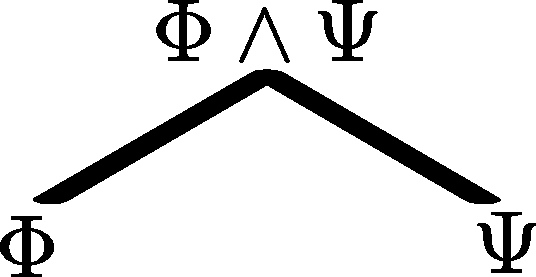
\includegraphics[scale=0.5]{andDiagram.pdf}\end{center}
Order does not matter for $\AND$; we consider $\pA\AND\pB$ and $\pB\AND\pA$ to be the same.


\paragraph{Disjunction}
\hypertarget{hl:OR}{Given} propositions $\pA$ and $\pB$, we can form their \emph{disjunction}
$$
\pA \OR \pB,
$$
which is expressed in English as ``$\pA$ or $\pB$.''
\hypertarget{hl:ORPV}{In} order to prove that $\pA\OR\pB$, you can either prove that $\pA$ or you can prove that $\pB$.
So if $\pA$ and $\pB$ happen to both hold, then you can still deduce that $\pA\OR\pB$
(unlike the way ``or'' is sometimes used in English).
The following diagram, showing what you can use to deduce $\pA\OR\pB$, kind of looks like the ``$\OR$'' symbol:
\begin{center}
\includegraphics[scale=0.5]{orDiagram.pdf}\end{center}
Order does not matter for $\OR$; we consider $\pA\OR\pB$ and $\pB\OR\pA$ to be the same.

If you know that $\pA\OR\pB$, then how can you use this fact in your arguments?
You cannot deduce $\pA$ and you cannot deduce $\pB$, so how do you proceed if you want to prove some other proposition $\pC$?
\hypertarget{hl:ORUSE}{The} rule that lets you proceed is called \emph{proof by cases}:
\RULE{Proof by cases}{
Suppose that you can prove $\pC$ by assuming $\pA$, and you can also prove $\pC$ by assuming $\pB$.
Then you can deduce $\pC$ from $\pA\OR\pB$.
}
In a written proof, the format of a proof by cases ends up like this:

\THMMOCK{Assuming that either $\pA$ or $\pB$ holds, we have $\pC$.}{
Assume that either $\pA$ or $\pB$ holds.\\
Case 1: Suppose that $\pA$ holds.
\indented{[insert argument here convincing the reader that $\pC$ holds]}
Case 2: Suppose that $\pB$ holds.
\indented{[insert argument here convincing the reader that $\pC$ holds]}
Since $\pC$ holds in both cases, we can conclude that $\pC$ holds.
}

Let's do an example using English sentences.
Suppose you see a plant with three-leaf bunches and you're sure that it's either poison ivy or poison oak, but you don't know which.
Well, you do know that poison ivy is poisonous and that poison oak is poisonous, so you can at least conclude that the plant you see is poisonous, even
if you don't know which type of plant it is.
That's a proof by cases.
To make the proof structure apparent in
the formatting given above, replace $\pA$ by ``the plant is poison ivy,'' replace $\pB$ by ``the plant is poison oak,'' and replace $\pC$ by ``the plant is poisonous.''

%You get something like this:
%\THM{Assuming that the plant is either poison ivy or poison oak, we can conclude that it is poisonous.}{
%Assume that the plant is either poison ivy or poison oak.\\
%Case 1: Suppose the plant is poison ivy.
%\indented{[insert argument convincing the reader that poison ivy is poisonous.]}
%Case 2: Suppose the plant is poison oak.
%\indented{[insert argument convincing the reader that poison oak is poisonous.]}
%Since the plant is poisonous either way, we can conclude that the plant is poisonous.
%}

\paragraph{Negation}
\hypertarget{hl:NOT}{Given} a proposition $\pA$, we can form its \emph{negation}
$$
\neg \pA,
$$
which is expressed in English as ``it is not the case that $\pA$.''
To prove $\neg\pA$ is to disprove $\pA$, and in fact this is what ``disprove'' means.
When $\pA$ holds we say that $\pA$ is \emph{true}, and when $\neg\pA$ holds we say that $\pA$ is \emph{false}.
We consider $\neg\neg\pA$ to be the same as $\pA$.

%It should never be the case that a proposition holds while its negation also holds.
%We hope, at least, that $\pA\AND\not\PA$ is not provable.
A proposition of the form $\pA\AND\neg\pA$ is called a \emph{contradiction}.
If something can both be and not be the case, then our entire deductive system is certainly broken.
We hope that no contradiction is provable in our language.
\hypertarget{hl:NOTPV}{This} leads us to accept the following as a way of proving a negation $\neg\pA$:
%Further, we explicitly deem contradictions to be \emph{impossible}, in the sense that any assumption
%that leads one to deduce a contradiction must be rejected as false.
%In order to prove that $\neg\pA$, you can assume that $\pA$ does hold and then show that this leads to a contradiction.
%This is called a \emph{proof by contradiction}:
\RULE{Proof by contradiction}{
If assuming $\pA$ allows you to deduce a contradiction, then it must be that $\neg\pA$.
}
In a written proof, the format of a proof by contradiction ends up like this:

\THMMOCK{$\neg\pA$.}{
Suppose, for the sake of obtaining a contradiction, that $\pA$ holds.
\indented{[insert argument convincing reader that a contradiction, something of the form $\pB\AND\neg\pB$, now follows]}
Since this is a contradiction, we conclude that $\neg\pA$.
}

Let's do an example using English sentences.
Say you're investigating a crime and you are considering a particular suspect.
Assuming the suspect did commit the crime, you can deduce that the suspect must have been at the crime scene on that day.
Upon questioning witnesses, you discover that the suspect was at work and could not have been at the crime scene that day.
This contradiction leads you to reject the original assumption; the suspect must not have committed the crime.
Making an assumption so that you can reject it after deducing an impossible situation-- that is a proof by contradiction.
To make the proof structure apparent in
the formatting given above, replace
$\pA$ by ``the suspect committed the crime'' and replace $\pB$ by ``the suspect was at the crime scene that day''.


The proof by contradiction rule rejects that a mathematical proposition can be both true and false.
There's
another rule involving negation which
enforces that mathematical propositions must be either true or false:
\RULE{Excluded middle}{
$\pA\OR\neg\pA$
}
There is no ``middle ground'' in which a proposition is neither true nor false.






% go back and do a better job presenting rules in terms of  formatting, and separatign susbsections perhaps with illustrated titles



% exercise that helps to understand how in english you can have inclusive and exclusive or, while math is inclusive.

% exercise that shows how parentheses are needed in and-or combinations
% in the same exercise you can show how and distributes over or and vice versa
% maybe the ex can be structured like this: for each of the following deductions, decide whether it is valid or not. if not valid, then justify by... 
  % uhhh truth table? or maybe you can give them some sample true and false english facts to put in, and do an example.

% some kind of exercise involving demorgan's law. or maybe you should write about that above
% idea: a deduction of demorgan's law going one way, and have them prove it going the other way

% maybe an exercise involving truth tables, having them fill one out for basic things and then for more complicated props

\ex{
The ``or'' of mathematical logic sometimes behaves differently from the English ``or.''
Describe a situation in which
\begin{center} ``The cake is flavored with either vanilla or chocolate.'' \end{center}
would pretty much be considered false, while
\begin{center} ``The cake is flavored with vanilla''\ $\OR$\ ``The cake is flavored with chocolate''. \end{center}
would be true.
}


\ex{
Suppose we know the following three facts:
\begin{itemize}
\item Whenever it rains over night, the grass gets wet. 
\item On a night that it doesn't rain, the sprinklers are run.
\item Whenever sprinklers are run, the grass gets wet.
\end{itemize}
Now write a proof of the following statement: ``The grass got wet last night.''
To make your argument, apply excluded middle to the statement ``It rained last night,''
and then do a proof by cases.
Follow the formatting given in this section for proof by cases.
}


\ex{
Suppose we know the following four facts:
\begin{itemize}
\item Whenever it rains over night, the grass gets wet. 
\item On a night that it doesn't rain, the sprinklers are run.
\item Whenever sprinklers are run, \emph{as long as they are not broken}, the grass gets wet.
\item The grass was dry last night.
\end{itemize}
Now write a proof of the following statement: ``It did not rain last night and the sprinklers are broken.''
To make your argument,
do a proof by contradiction to establish ``it did not rain last night,''
and do another proof by contradiction to establish ``the sprinklers are broken.''
Once both are established you can conclude the conjunction.
Follow the formatting given in this section for proof by contradiction.
}





\newcommand{\truthtablefour}[5]{
\begin{tabular}{|c|c|c|}
\hline
$\pA$ & $\pB$ & #1 \\ \hline
F     & F  & #2   \\ \hline
F     & T  & #3   \\ \hline
T     & F  & #4   \\ \hline
T     & T  & #5   \\ \hline
\end{tabular}
}

\newcommand{\truthtabletwo}[3]{
\begin{tabular}{|c|c|}
\hline
$\pA$ & #1 \\ \hline
F     & #2   \\ \hline
T     & #3   \\ \hline
\end{tabular}
}


\def\sp{\hspace{1em}}

\ex{
Thanks to the law of excluded middle, there are only two possibilities for a single proposition $\pA$: it is either true or false.
For \emph{two} propositions $\pA$ and $\pB$, there are \emph{four} possibilities, which we can list in a nice table:
\begin{center}
\begin{tabular}{|c|c|}
\hline
$\pA$ & $\pB$ \\ \hline
F     & F     \\ \hline
F     & T     \\ \hline
T     & F     \\ \hline
T     & T     \\ \hline
\end{tabular}
\end{center}
For three propositions there are eight possibilities, and so on.
This suggests a useful way to think about the logical operators $\AND$, $\OR$, and $\neg$:
\begin{center}
\truthtablefour{$\pA\AND\pB$}{F}{F}{F}{T}
\sp
\truthtablefour{$\pA\OR\pB$}{F}{T}{T}{T}
\sp
\truthtabletwo{$\neg\pA$}{T}{F}
\end{center}
Here we are simply listing all the possibilities for the component propositions $\pA$, $\pB$, etc.,
and then we are indicating whether the complex proposition is true or false in each case. These are called \emph{truth tables}.
\begin{enumerate}
\item
Write out a truth table for $\neg(\pA\AND\pB)$. It should have four rows.

\item
Write out a truth table for $(\pA\AND\pB)\OR\pC$, and also for $\pA\AND(\pB\OR\pC)$.
The table should have eight rows, and you can feel free to make just one table in which 
there is a column for $(\pA\AND\pB)\OR\pC$ and a column for $\pA\AND(\pB\OR\pC)$.

\item
Your answer to the above should convince you that it's a terrible idea to write something like ``$\pA\AND\pB\OR\pC$.''
Replace $\pA$, $\pB$, and $\pC$ by English sentences in $\pA\AND\pB\OR\pC$ such that you get an ambiguous Enlgish sentence.
Explain the ambiguity in your sentence.

\item \label{itm:truthtables:first_equiv}
Write out a truth table for $(\pA\AND\pB)\AND\pC$, and also for $\pA\AND(\pB\AND\pC)$.
The answer should convince you that there is no trouble at all with writing $\pA\AND\pB\AND\pC$,
though you were probably convinced anyway since $\pA\AND\pB\AND\pC$ can obviously only mean:
``$\pA$, $\pB$, and $\pC$ are all true.''

\item
Write out a truth table for $(\pA\AND\pB)\OR\pA$. This one should just have four rows.
Looking at the table, do you see a way to ``simplify'' the complex proposition  $(\pA\AND\pB)\OR\pA$?

\item
Write out a truth table for $(\pA\AND\pB)\OR\pC$, and also for $(\pA\OR\pC)\AND(\pB\OR\pC)$.
This should show you that $\OR$ can ``distribute'' over $\AND$.

\item
Write out a truth table for $(\pA\OR\pB)\AND\pC$, and also for $(\pA\AND\pC)\OR(\pB\AND\pC)$.
This should show you that $\AND$ can ``distribute'' over $\OR$.

\item \label{itm:truthtables:last_equiv}
Write out a truth table for $\neg(\pA\AND\pB)$, and also for $(\neg\pA)\OR(\neg\pB)$.
\end{enumerate}
In parts \ref{itm:truthtables:first_equiv} through \ref{itm:truthtables:last_equiv},
you see that certain propositions are ``equivalent'' in some sense. The formal meaning of ``equivalent'' will be
discussed in the next section.
}


\subsubsection{If and Iff}

\paragraph{Implication}
\hypertarget{hl:ARR}{Given} propositions $\pA$ and $\pB$, we can form the \emph{implication}
$$
\pA\ARR\pB,
$$
which is expressed in English as ``$\pA$ implies $\pB$'' or ``if $\pA$, then $\pB$.''
The ``$\pA$'' part of an implication $\pA\ARR\pB$ is called the \emph{hypothesis},
and the ``$\pB$'' part is called the \emph{conclusion}.
\hypertarget{hl:ARRPV}{To} prove $\pA\ARR\pB$,
start by assuming $\pA$ and
then give an argument that $\pB$ follows.
That is, assume the hypotheses and then argue that the conclusion follows.
Such a proof ends up structured like this:

\THMMOCK{If $\pA$, then $\pB$.}{
Assume that $\pA$.
\indented{[insert argument convincing reader that $\pB$ holds]}
Thus, $\pA\ARR\pB$.
}

\hypertarget{hl:ARRUSE}{The} rule that allows us to use $\pA\ARR\pB$ is modus ponens:
\RULE{Modus ponens}{
Given $\pA\ARR\pB$ and $\pA$, you can deduce $\pB$.
}
Here is also another great rule for using an implication (this one can be derived from modus ponens via a proof by contradiction):
\DRULE{Modus tollens}{
Given $\pA\ARR\pB$ and $\neg\pB$, you can deduce $\neg\pA$.
}

\paragraph{Logical Equivalence}
\hypertarget{hl:DARR}{Given}  propositions $\pA$ and $\pB$, we can form the \emph{logical equivalence}
$$
\pA\DARR\pB,
$$
which is expressed in English as ``$\pA$ if and only if $\pB$,'' often shortened to ``$\pA$ iff $\pB$.''

An equivalence holds when two propositions are forced to be true or false \emph{together}--
that is, when they are either both true or both false.

\hypertarget{hl:DARRPV}{To} prove an equivalence $\pA\DARR\pB$, simply prove both of the implications $\pA\ARR\pB$ and $\pB\ARR\pA$.
The proof will be structured like this:

\THMMOCK{$\pA\DARR\pB$.}{
Assume that $\pA$.
\indented{[insert argument convincing reader that $\pB$ holds]}
Now assume that $\pB$.
\indented{[insert argument convincing reader that $\pA$ holds]}
}

\hypertarget{hl:DARRUSE}{Using} an equivalence works a lot like modus ponens, except it goes in both directions.
If you know that $\pA\DARR\pB$, then you can deduce $\pA$ from $\pB$, $\neg\pA$ from $\neg\pB$,
$\pB$ from $\pA$, and $\neg\pB$ from $\neg\pA$.



\def\sp{\hspace{1em}}

Here are the truth tables for $\ARR$ and $\DARR$:
\begin{center}
\truthtablefour{$\pA\ARR\pB$}{???}{???}{F}{T}
\sp
\truthtablefour{$\pA\DARR\pB$}{T}{F}{F}{T}
\end{center}
There should be nothing surprising there, except that I've left some question marks in position where I think you might be surprised.
If $\pA$ is false, then what of the proposition $\pA\ARR\pB$?
It has to be either true or false (due to excluded middle), so which is it?
Put another way: Suppose you say ``If $3$ is even, then $3$ is divisible by $2$.''
Knowing that $3$ is not even, are you a liar? Is your statement true or false?
The answer is that it's \emph{true}!
Here is the completed truth table for $\ARR$:
\begin{center}
\truthtablefour{$\pA\ARR\pB$}{T}{T}{F}{T}
\end{center}
Putting T there is not an arbitrary choice-- if you agreed with all the previous logical rules then you \emph{must} agree
that $\pA\ARR\pB$ is \emph{true} when $\pA$ is false.
Let me try and convince you. First we need to revisit contradictions.


\def\vsp{\\[0.5em]}

Recall how \emph{proof by contradiction} works:
If an assumption leads to a contradiction, then the assumption is rejected as false.
If you assume $\pB$, and then after some argumentation you deduce $\pA\AND\neg\pA$, then
you can back out of your original assumption and conclude without a doubt that $\neg\pB$.
Now let's think, hypothetically, what would happen if a contradiction $\pA\AND\neg\pA$ were actually \emph{true}?
If $\pA\AND\neg\pA$ holds, then we can prove $\pB$ by contradiciton as follows:
\indented{
Suppose, for the sake of contradiction, that $\neg\pB$ holds.\vsp
Since $\pA\AND\neg\pA$ has already been assumed to hold, we've already reached a contradiction.\vsp
We conclude that $\neg\neg\pB$, and therefore $\pB$, must hold.
}
Let's be clear about what just happened: from the assumption $\pA\AND\neg\pA$, we were able to prove an \emph{arbitrary proposition}!
This mechanism was always present in the proof by contradiction rule, but it is worth highlighting:

\DRULE{\label{rule:contradictions}Contradictions are powerful!}{
From $\pA\AND\neg\pA$ you can deduce \emph{any} proposition $\pB$.
}

Now back to the question of how to treat $\pA\ARR\pB$ when $\pA$ is false.
Recall that in order to prove $\pA\ARR\pB$, one can assume $\pA$ and then deduce $\pB$.
If we know that $\pA$ is false to start with, then here is a proof that $\pA\ARR\pB$:
\indented{
Assume $\pA$.\vsp
Since $\pA$ is known to be false, we now have a contradiction $\pA\AND\neg\pA$.\vsp
Using ``contradictions are powerful,'' we can now deduce anything we want! In particular, we can deduce $\pB$.
}
Thus if you accept proofs by contradiction as valid, then you must accept that $\pA\ARR\pB$ is true when $\pA$ is false.
An implication that is true because its hypothesis is false is sometimes said to be \emph{vacuously true}.

\ex{
Assume that we know the following facts:
\begin{itemize}
\item Alice is an accountant and holds no other profession.
\item Bob has brown hair.
\item Charles loves chocolate and despises all other foods.
\end{itemize}
Determine whether each of the following is true or false.
\begin{enumerate}


\item %3
If
Bob's hair is purple
then
Charles loves chocolate.


\item %2
If
Alice is an accountant
then
Charles likes green beans.


\item %6
Alice is an accountant
if and only if
Alice is a doctor.


\item %1
If
Bob has brown hair
then
Charles loves chocolate.


\item %7
Charles likes baked salmon
if and only if
Bob has brown hair.


\item %8
Charles likes clam chowder
if and only if
Alice is a professional underwater welder.

\item %4
If
Bob's hair is green
then
Bob's hair is white.

\item %5
Bob's hair is brown
if and only if
Charles loves chocolate.


\end{enumerate}

Notice how the implication of mathematical logic has nothing to do with causality.
Some of the sentences above sound weird in English because we often use ``if... then...'' to 
indicate that one state of affairs \emph{causes} another, as in the sentence
\begin{center}``If you don't brush your teeth, then you will get cavities.''\end{center}
In mathematical logic, that sentence is simply true if you either brush your teeth, or if you don't brush your teeth and end up getting cavities.
Interestingly, that sentence is true even in a situation where you brush your teeth and still get cavities.
That's quite different from the ``if... then...'' of conversational English!
In conversation, we would expect there to be an implicit
\begin{center}``(And if you do brush your teeth then you will not get cavities.)''\end{center}
Be aware that this implicit additional statement is not there in mathematical logic; 
an implication $\pA\ARR\pB$ doesn't give you any information in the case where you know that $\neg\pA$.
}

\ex{
Write a truth table for $(\pA\ARR\pC)\AND(\pB\ARR\pC)$. It should have eight rows.
In the same truth table, add a column for $(\pA\OR\pB)\ARR\pC$.
Finally, in the same truth table, add a column for 
$$((\pA\ARR\pC)\AND(\pB\ARR\pC))\ARR((\pA\OR\pB)\ARR\pC).$$
The latter proposition could be called ``proof by cases,'' and so your truth table result should not be too surprising.
}

\subsubsection{Some Derived Logical Rules}
\label{sec:derived1}

In this section we will derive some logical rules from the basic ones given in previous sections.
We still have no specific mathematical propositions to talk about and so we still use the placeholders $\pA$, $\pB$, etc.
The arguments given in this section are useful logical patterns that can help us build other arguments later on.

The following derived rule could be written as ``$((\pA\ARR\pB)\AND(\pB\ARR\pC))\ARR(\pA\ARR\pC)$'',
but we instead mix in some English to cut down on the number of parentheses and to make things more pleasant to read.

\DRULEPF{Transitivity of Implication}{
If $\pA\ARR\pB$ and $\pB\ARR\pC$, then $\pA\ARR\pC$.
}{
Assume that $\pA\ARR\pB$ and $\pB\ARR\pC$.
In order to prove that $\pA\ARR\pC$, let us assume $\pA$.
(Our goal is now to prove $\pC$.)
From $\pA$ and $\pA\ARR\pB$, it follows that $\pB$.
From $\pB$ and $\pB\ARR\pC$, it follows that $\pC$.
}

In the above argument you can see two applications of modus ponens-- this is how implications can be put to use.
And you can also see how an implication is proven, by assuming the hypotheses and arguing for the conclusion.

\def\lsp{\\[-0.4em]}

\DRULEPF{Conjunction and Implication}{
$(\pA\AND\pB)\ARR\pC$ if and only if $(\pA\ARR(\pB\ARR\pC))$
}{
Assume that $(\pA\AND\pB)\ARR\pC$.
In order to prove $(\pA\ARR(\pB\ARR\pC))$, assume $\pA$.
Now in order to prove $\pB\ARR\pC$, assume $\pB$.
Since we have both $\pA$ and $\pB$, we have $\pA\AND\pB$.
Since $(\pA\AND\pB)\ARR\pC$, we can now conclude $\pC$.\lsp

Now assume that $(\pA\ARR(\pB\ARR\pC))$.
In order to prove that $(\pA\AND\pB)\ARR\pC$,
assume $\pA\AND\pB$.
That is, we have assumed $\pA$ and we have assumed $\pB$.
From $\pA$ and $\pA\ARR(\pB\ARR\pC)$, it follows that $\pB\ARR\pC$.
From $\pB$ and $\pB\ARR\pC$, it follows that $\pC$.
}

The first thing to notice about the above argument is the way in which an ``if and only if'' statement gets proven.
There are two parts to the proof, one for each of the two implications.
The first half of the proof establishes 
$$((\pA\AND\pB)\ARR\pC)\ARR((\pA\ARR(\pB\ARR\pC))),$$
while the second half establishes
$$((\pA\ARR(\pB\ARR\pC)))\ARR((\pA\AND\pB)\ARR\pC).$$
Together, they allow us to conclude the ``if and only if'' statement
$$((\pA\AND\pB)\ARR\pC)\DARR((\pA\ARR(\pB\ARR\pC))).$$
Another thing to notice is the way in which $\AND$ is handled.
In the first half of the argument, we establish that $\pA\AND\pB$ holds by establishing each of $\pA$ and $\pB$-- this is the way to prove a conjunction.
In the second half, we get to assume that $\pA\AND\pB$ holds and this allows us to deduce both $\pA$ and $\pB$-- this is the way conjunctions get used.
In typical proofs this handling of conjunctions happens very quickly; the distinction between
\begin{center} ``Assume that $\pA\AND\pB$''\end{center}
and
\begin{center} ``Assume that $\pA$ and assume that $\pB$''\end{center}
will be blurred completely.

\DRULEPZ{}{If $\pA\ARR\pB$ and $\pC\ARR\pD$, then $(\pA\AND\pC)\ARR(\pB\AND\pD)$.}

\DRULEPF{Disjunction and Implication}{
$(\pA\OR\pB)\ARR\pC$ if and only if $(\pA\ARR\pC)\AND(\pB\ARR\pC)$
}{
$\Rightarrow$:
Assume that $(\pA\OR\pB)\ARR\pC$.
\lsp

In order to prove that $(\pA\ARR\pC)$, assume $\pA$.
From $\pA$ it follows that $\pA\OR\pB$.
From $\pA\OR\pB$ and $(\pA\OR\pB)\ARR\pC$, we can conclude that $\pC$.
Thus we have proven that $\pA\ARR\pC$.
\lsp

We also need to prove that $\pB\ARR\pC$. To this end, assume $\pB$.
From $\pB$ it follows that $\pA\OR\pB$.
From $\pA\OR\pB$ and $(\pA\OR\pB)\ARR\pC$, we can conclude that $\pC$.
Thus we have proven that $\pB\ARR\pC$.
\lsp

Since we proved $\pA\ARR\pC$ and $\pB\ARR\pC$, we can conclude that $(\pA\ARR\pC)\AND(\pB\ARR\pC)$.
\lsp

$\Leftarrow$: 
Assume that $(\pA\ARR\pC)\AND(\pB\ARR\pC)$.
That is, assume  $\pA\ARR\pC$ and assume $\pB\ARR\pC$.
For the sake of proving $(\pA\OR\pB)\ARR\pC$, assume that $\pA\OR\pB$.
\lsp

Case 1: In the case that $\pA$ holds, it follows from $\pA\ARR\pC$ that $\pC$ holds.
\lsp

Case 2: In the case that $\pB$ holds, it follows from $\pB\ARR\pC$ that $\pC$ holds.
\lsp

Since $\pC$ holds in both cases, we conclude that $\pC$ holds.
}

Here the two halves of the ``if and only if'' proof are difficult to separate by paragraphs alone, since each half needed multiple paragraphs.
So the two halves of the proof are headed by ``$\Rightarrow$'' and ``$\Leftarrow$''.
You should always feel free to use headings to separate different components of your argument.

Another thing to notice in the above argument is the way in which $\OR$ is handled.
In the first half of the argument, we establish $\pA\OR\pB$ by deducing it from $\pA$, and we also establish it by deducing it from $\pB$.
In the second half, we use an $\OR$ statement in pretty much the only way we can-- a proof by cases.

\DRULEPZ{}{If $\pA\ARR\pB$ and $\pC\ARR\pD$, then $(\pA\OR\pC)\ARR(\pB\OR\pD)$.}

\DRULEPF{Alternative Eliminated}{
If $\pA\OR\pB$ holds but $\pA$ does not hold, then $\pB$ must hold.
In other words,
$$((\pA\OR\pB)\AND(\neg\pA))\ARR\pB.$$
}{
Assume that $\pA\OR\pB$ holds and $\neg\pA$ holds.
\lsp

Case 1: Suppose that $\pA$ holds.
Then we have $\pA\AND\neg\pA$! From a contradiction we can conclude anything, in particular we can conclude that $\pB$ holds.
\lsp

Case 2: Suppose that $\pB$ holds... that's it for case 2.
\lsp

In both cases we conclude $\pB$, so we can conclude $\pB$.
}

In the above argument we've made use of the previously discussed rule ``contradictions are powerful!''


\DRULEPF{Or Distributes over And}{
$(\pA\OR(\pB\AND\pC))\DARR((\pA\OR\pB)\AND(\pA\OR\pC))$.
}{
$\Rightarrow$:
Assume $\pA\OR(\pB\AND\pC)$.
\lsp

Case 1: Suppose $\pA$ holds. Then we can immediately conclude $\pA\OR\pB$ and $\pA\OR\pC$, and from these
we can conclude $(\pA\OR\pB)\AND(\pA\OR\pC)$.
\lsp

Case 2: Suppose $\pB\AND\pC$ holds.
Then $\pB$ holds, and $\pA\OR\pB$ then follows from that.
Also $\pC$ holds, and $\pA\OR\pC$ follows from that.
Finally we conclude $(\pA\OR\pB)\AND(\pA\OR\pC)$.
\lsp

Since both cases lead to $(\pA\OR\pB)\AND(\pA\OR\pC)$, we conclude $(\pA\OR\pB)\AND(\pA\OR\pC)$.
\lsp

$\Leftarrow$: Assume $((\pA\OR\pB)\AND(\pA\OR\pC))$.
That is, assume $\pA\OR\pB$ and assume $\pA\OR\pC$.
Due to excluded middle, we know that either $\pA$ or $\neg\pA$ holds.
\lsp

Case 1: Suppose that $\pA$ holds. It immediately follows that $\pA\OR(\pB\AND\pC)$.
\lsp

Case 2: Suppose that $\neg\pA$ holds. Using the rule ``alternative eliminated,''
it then follows from $\pA\OR\pB$ that $\pB$ holds.
Similarly, it follows from $\pA\OR\pC$ that $\pC$ holds. Thus $\pB\AND\pC$ holds.
Finally, we conclude that $\pA\OR(\pB\AND\pC)$.
\lsp

Since both cases lead to $\pA\OR(\pB\AND\pC)$, we conclude $\pA\OR(\pB\AND\pC)$.
}

Observe that a proof by cases need not proceed from the exact $\OR$-proposition one has assumed;
sometimes it is useful to do a proof by cases based on excluded middle.

%\DRULEPZ{And Distributes over Or}{
%$(\pA\AND(\pB\OR\pC))\DARR((\pA\AND\pB)\OR(\pA\AND\pC))$.
%}
%
%The following rule was actually already used in an argument in the previous section.
%It's interesting to see that this rule can be derived from prior rules.
%
%\DRULEPF{Double Negation}{
%$\pA\DARR(\neg\neg\pA)$.
%}{
%Assume $\pA$. Assume, for the sake of obtaining a contradiction, that $\neg\pA$.
%Then we immediately have a contradiction $\pA\AND\neg\pA$, and so we conclude that $\neg\neg\pA$.
%\lsp
%
%Now assume $\neg\neg\pA$.
%Our goal is to prove $\pA$.
%Due to excluded middle, we have that $\pA\OR\neg\pA$.
%In the case that $\pA$ holds, we are done with the proof. 
%In the case that $\neg\pA$ holds, we have the contradiction 

%% THIS IS CIRCULAR! The problem is that Contradictions are Powerful was supposed to be an axiom, and I'm using proof by contradiction as an axiom instead.
%% Proof by contradiction only allows you to prove negations.

%}








% Define notions of converse, inverse, and contrapositive.
Given an implication $\pA\ARR\pB$, there are a few ``flipped'' implications one can write down:
\indented{The \emph{converse} of $\pA\ARR\pB$ is $\pB\ARR\pA$.\\
          The \emph{inverse} of $\pA\ARR\pB$ is $\neg\pA\ARR\neg\pB$.\\
          The \emph{contrapositive} of $\pA\ARR\pB$ is $\neg\pB\ARR\neg\pA$.}
It is a common mistake to think that the converse or the inverse of an implication follows from the implication.
The confusion stems from the inconsistent ways in which ``if... then...'' can work in conversation.
When a bank robber says
\begin{center}
``If you don't hand over the money, I'll shoot!'',
\end{center}
they implicitly also mean to say the inverse
\begin{center}
``If you do hand over the money, then I won't shoot!'',
\end{center}
and the converse
\begin{center}
``I'll shoot only if you don't hand over the money!''
\end{center}
If the bank robber were using strict mathematical logic (that is, if their original
threat took the form ``you don't hand over the money''$\ARR$``I will shoot''), then
they could, without lying, shoot even after the money is handed over.

The \emph{contrapositive} of an implication, on the other hand, \emph{does} follow from the implication.
This rule is derived below.
An implication is always equivalent to its contrapositive.
Since the converse of an implication is the contrapositive of its inverse, the converse and inverse of an implication are equivalent.






% Prove that impliation holds iff contrapositive does.
\DRULEPF{Contraposition\label{drule:contraposition}}{$(\pA\ARR\pB)\DARR(\neg\pB\ARR\neg\pA)$}{
Assume that $\pA\ARR\pB$.
To prove that $\neg\pB\ARR\neg\pA$, assume that $\neg\pB$.
Now assume $\pA$, for the sake of obtaining a contradiction.
Since $\pA\ARR\pB$, we see that $\pB$ follows. We end up with the contradiction $\pB\AND\neg\pB$.
Thus we reject the original assumption and conclude that $\neg\pA$.
\lsp

Now to prove the other direction, assume that $\neg\pB\ARR\neg\pA$.
To prove that $\pA\ARR\pB$, assume $\pA$.
For the sake of obtaining a contradiction, assume $\neg\pB$.
From $\neg\pB\ARR\neg\pA$, it then follows that $\neg\pA$.
But we've now reached the contradiction $\pA\AND\neg\pA$.
Thus we reject the original assumption and conclude that $\neg\neg\pB$.
In other words, $\pB$.
}

% Comment on how pf by contradiction appears as a great tool for disproving something.
The above argument is a great demonstration of how proofs by contradiction work.
Sometimes, in order to proceed with your argument, you need something \emph{more} to work with.
Assuming that your desired conclusion doesn't hold can sometimes give you something more and help push your argument forward.

The above argument should make you feel that ``proof by contradiction'' and ``contraposition'' are very closely related.
%The theorems you prove will most often take the form of an implication, something like
%\begin{center}If $\pA$, $\pB$, and $\pC$, then $\pD$. \end{center}
One can prove $\pA\ARR\pB$ by assuming $\pA$, then assuming $\neg\pB$ and trying to obtain a contradiction.
Or, one can prove $\pA\ARR\pB$ by instead proving its contrapositive $\neg\pB\ARR\neg\pA$, which we now see is equivalent to the original implication.
Both approaches amount to pretty much the same argument.

\vspace{1em}

\DRULEPF{Inverting an Equivalence\label{drule:neg_equiv}}{
If $\pA\DARR\pB$, then $\neg\pA\DARR\neg\pB$.
}{
Assume that $\pA\DARR\pB$. Then $\pA\ARR\pB$ and $\pB\ARR\pA$.
By contraposition, it follows that $\neg\pB\ARR\neg\pA$ and $\neg\pA\ARR\neg\pB$.
Thus we have $\neg\pA\DARR\neg\pB$.
}

% do LXXXIII ii
\DRULEPF{De Morgan's Law 1\label{drule:demorgan1}}{$\neg(\pA\AND\pB)\ \DARR\ (\neg\pA\OR\neg\pB)$}{
$\Rightarrow$: Assume $\neg(\pA\AND\pB)$.
Due to excluded middle, either $\pA$ or $\neg\pA$.\lsp

Case 1: Suppose that $\pA$ holds. Now if $\pB$ held we would obtain $\pA\AND\pB$, which leads to the contradiction $(\pA\AND\pB)\AND\neg(\pA\AND\pB)$.
Therefore it must be that $\neg\pB$. From this it follows that $\neg\pA\OR\neg\pB$.\lsp

Case 2: Suppose that $\neg\pA$ holds. Then it immediately follows that $\neg\pA\OR\neg\pB$.
Since we ended up with $\neg\pA\OR\neg\pB$ in both cases, we can conclude that $\neg\pA\OR\neg\pB$.
\\[1em]

$\Leftarrow$: Assume $(\neg\pA)\OR(\neg\pB)$.
Suppose, for the sake of contradiction, that $\pA\AND\pB$ holds.
Then $\pA$ holds, and $\pB$ holds. Since we know that $(\neg\pA)\OR(\neg\pB)$ holds, there are two cases to consider:\lsp

Case 1: Suppose that $\neg\pA$ holds. Then, since we already said that $\pA$ holds, we obtain the contradiction $\pA\AND\neg\pA$.\lsp

Case 2: Suppose that $\neg\pB$ holds. Then, since we already said that $\pB$ holds, we obtain the contradiction $\pB\AND\neg\pB$.\lsp

We obtain a contradiction either way, and so we are forced to reject that $\pA\AND\pB$. That is, we have $\neg(\pA\AND\pB)$.
}



% puzzle LXXXIII i
\DRULEPZ{De Morgan's Law 2\label{drule:demorgan2}}{
$\neg(\pA\OR\pB)\ \DARR\ (\neg\pA\AND\neg\pB)$
}


% do LXXXVII i but make the forward direction a puzzle, with hint to use excluded middle
\DRULEPF{Implication in Terms of Disjunction\label{drule:unless}}{
$(\pA\ARR\pB)\DARR(\neg\pA\OR\pB)$
}{
$\Rightarrow$: \putExerciseHeading: Prove that $(\pA\ARR\pB)\ARR(\neg\pA\OR\pB)$. Hint: Use excluded middle.
\lsp

$\Leftarrow$: Assume that $\neg\pA\OR\pB$. With the goal of proving that $\pA\ARR\pB$, assume that $\pA$.
Applying the previous rule ``alternative eliminated,''
we can conclude $\pB$ from $\neg\pA\OR\pB$ and $\pA$.
}

% comment on the inutiitiveness of this as ``$\pB$, unless $\neg\pA$'', and on how it means implications were not needed
The fact that $\pA\ARR\pB$ can be rewritten as $\neg\pA\OR\pB$ suggests that we never needed to formally introduce $\ARR$ into our language.
Everytime we want to say ``if $\pA$, then $\pB$,'' we could instead say ``either $\pB$, or it's not the case that $\pA$.''
But life is better when we can phrase things in terms of $\ARR$, and that is why we choose to have it.

% puzzle $\neg(\pA\ARR\pB)\DARR (\pA\AND\neg\pB)$
\DRULEPZ{Negating an Implication\label{drule:neg_impl}}{$\neg(\pA\ARR\pB)\DARR (\pA\AND\neg\pB)$}

% comment that it's important to understand this so that we know how to negate logical statements by ``pushing'' the $\neg$ inside things. demorgan tells us how to deal with $\AND$ and $\OR$.
The rule above and De Morgan's laws give you a way ``push'' a negation $\neg$ into complicated propositions. This will really come in handy later on!
For example,
negating $\pA\ARR(\pB\OR\pC)$
initially yields $\neg(\pA\ARR(\pB\OR\pC))$, but after pushing the negation in it becomes 
$\pA\AND\neg(\pB\OR\pC)$.
After pushing the negation in further this becomes $\pA\AND\neg\pB\AND\neg\pC$.

\ex{
Negate each of the following propositions, and push the negation into the innermost component propositions.
\begin{enumerate}
\item
$\pA\ARR(\pB\OR\pC)$
\item
$((\pA\OR\pB)\ARR\pC)\AND\pD$
\item
If you eat right and you sleep well, then you are healthy and you will live long.
\end{enumerate}
}


% final comment: the purpose of derived rules to show us common patterns of proofs and to strengthen our sense for mathematical logic.
% typically we do not use these rules directly in a hyperrigid proof structure, but rather we rely on our sense for mathematical logic.
% it is important that this sense be sufficiently developed to write correct proofs, especially important that we be aware how it's different from plain conversation.
The main purpose of the derived rules in this section is to make us familiar with common patterns of proofs.
Typically we do not reference these rules directly, but rather we rely on our intuitive sense for mathematical logic to enable us to read mathematical arguments and to
construct our own arguments.
A second purpose of this section is to help strengthen that intuitive sense for mathematical logic,
which really must be sufficiently developed in order for us to write correct proofs.
It is especially important to be aware of the ways in which mathematical logic differs from the sometimes ambiguous logic of everyday conversation.


% introduce some kind of reasonable exercise numbering and formatting. Proofread.

% consider putting a summary of "rules" somewhere...






% use jacoby notes as a guide, but also look at ``thinking about logic'', and also show a truth table and point out the weird part.
% pull out my old psychology course final paper as well

\subsubsection{Substitution}
\label{sec:subst}

Our entire discussion has so far been restricted to propositions, but for the next part \emph{variables} will have a role to play.
Before moving on, review section
\ref{sec:parts_of_speech} as needed to remind yourself about variables, constants, terms, and propositions.

\newcommand{\eg}[4]{If $\pA$ is ``#1'' then $\SUBST{\pA}{#2}{#3}$ is ``#4''.}
\def\lsp{\\[0.4em]}

Given a proposition $\pA$, the notation
$$
\SUBST{\pA}{x}{T}
$$
stands for the proposition that is obtained by replacing each ``$x$'' in $\pA$ with a ``$T$''.
In this notation, any variable can go in the position of ``$x$'' and any term can go in the position of ``$T$'':
\begin{center}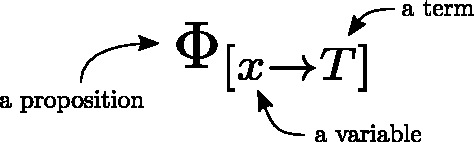
\includegraphics[scale=0.8]{subst.pdf}\end{center}
Some examples:
\indented{
\eg{$x\in A\cup B$}{x}{y}{$y\in A\cup B$}\lsp
\eg{$x\in A\cup B$}{A}{x}{$x\in x\cup B$}\lsp
\eg{$z^2=z+y$}{z}{a+y}{$(a+y)^2=(a+y)+y$}\lsp
\eg{$a+b\in B$}{c}{3}{$a+b\in B$}\lsp
\eg{the product of $a$ and $b$ is even}{b}{c^2}{the product of $a$ and $c^2$ is even}
}
\paragraph{A Clarification}
(If you find this remark to be more confusing than clarifying, then please feel free to skip this paragraph for now.)
What \emph{is} the string of symbols ``$\SUBST{\pA}{x}{T}$''? What part of speech are we looking at here?
It's almost a proposition, in that you get a proposition once you carry out the substitution that involves replacing $x$ by $T$.
But the string of symbols ``$\SUBST{\pA}{x}{T}$'' is not itself a proposition.
It's more like a set of \emph{instructions} telling you how to obtain a certain proposition.
The string of symbols ``$\SUBST{\pA}{x}{T}$''
has no part of speech because it is in fact not a part of the mathematical language at all!
Instead, it is part of the language we are currently using to communicate. That is, it is a part of the English
language in which this document is written, and it will help us in our mission to \emph{specify} the language of mathematics.
You can think of ``$\SUBST{\pA}{x}{T}$'' as simply a shorthand for the instruction 
\indented{
\emph{Take the proposition ``$\pA$'' and replace all occurances of the variable ``$x$'' with the term ``$T$'', and then write the resulting proposition.}
}

\paragraph{More on substitution is coming later.}
There is a little more to substitution than simple mechanical replacement of symbols.
I've left out some important details in this section.
Take a look at these examples:
\indented{
\eg{$\ALL{x}{x=2}$}{x}{y}{$\ALL{x}{x=2}$}\lsp
\eg{$(x\in A)\AND\EXIST{x}{x=2}$}{x}{y}{$(y\in A)\AND\EXIST{x}{x=2}$}\lsp
\eg{$a\in \COLL{a}{a^2=z}$}{a}{3}{$3\in \COLL{a}{a^2=z}$}
}
In these examples, substitution does not work as you might expect. 
You might guess from the examples that the barbell symbol ``$\bbel$'' has a hand in the strange substitution rules.
We are not ready to dig into these details just yet. Later
in section \ref{sec:subst_again}, there will be more on ``$\bbel$'' and its effect on substitution.
For now, rest assured that the substitutions in the upcoming exercise are all straightforward ones--
there will be no funny business with barbells.


\ex{
For each of the following, write the proposition that results from the substitution.
\begin{enumerate}
\item $\SUBST{\text{``\ $\frac{a+b}{x+y}>x^2$\ ''}}{x}{A+B}$
\item $\SUBST{\text{``\ $B\neq B$\ ''}}{B}{y}$
\item $\SUBST{\text{``\ $z\in\{\alpha,\beta,\gamma\}$\ ''}}{\beta}{\gamma^{-1}}$
\item $\SUBST{\text{``\ $f\subseteq A\times B$\ ''}}{f}{g\circ f}$
\item $\SUBST{\text{``\ $x\in y\ARR x\in z$\ ''}}{x}{3}$
\item $\SUBST{\text{``\ $a=2\OR a=3$\ ''}}{b}{5}$
\item $\SUBST{\pB}{b}{5}$, where $\pB$ is the proposition ``$b\times b\subseteq J$''
\item $\SUBST{\text{``\ $n^2$ is even\ ''}}{n}{1}$
\item $\SUBST{\text{``\ $n^2$ is even\ ''}}{n}{n+1}$
\item $\SUBST{\SUBST{\text{``\ $n^2\sim k$\ ''}}{n}{j+k}}{k}{3}$
\end{enumerate}
}

\ex{
Is $\SUBST{\SUBST{\pA}{x}{y}}{y}{x}$ always the same as $\pA$? Explain.
}




\subsubsection{Universal and Existential Quantifiers}

\def\lsp{\\[0.3em]}
\newcommand{\EGENTRY}[2]{#1\hspace{1em} & #2\lsp}

\paragraph{Universal Quantifiers}
\hypertarget{hl:UQ}{Given} a proposition $\pA$ and a variable $x$, we can form
the \emph{universally quantified} proposition
$$
\ALL{x}{\pA},
$$
which is expressed in English as ``for all $x$, $\pA$.''
Typically the proposition $\pA$ would somehow involve the variable $x$.
Here are some examples, along with their expressions in English:
\indented{
\begin{tabular}{ll}
\EGENTRY{
$\ALL{x}{x=x}$
}{
For all $x$, $x=x$.
}
\EGENTRY{
$\ALL{n}{n>x}$
}{
For all $n$, $n>x$.
}
\EGENTRY{
$\ALL{y}{\text{($y$ is green)}\AND\text{($y$ is a flower)}}$
}{
For all $y$, $y$ is green and $y$ is a flower.
}
\EGENTRY{
$\ALL{y}{\text{($y$ is a flower)}\ARR\text{($y$ is green)}}$
}{
For all $y$, if $y$ is a flower then $y$ is green.
}
\end{tabular}
}

\def\BLANK{\underline{\hspace{8pt}}}

In each proposition, the variable behind the ``$\bbel$'' is said to be \emph{quantified}.
The quantified variable is special in that it's really just a placeholder.
The proposition ``$\ALL{x}{x=x}$'' is no different from
``$\ALL{y}{y=y}$''.
We might as well write them both as as
``$\ALL{\BLANK}{\BLANK=\BLANK}$'',
with the understanding that the blanks all refer to the same thing.
It is always possible to express universally quantified propositions in English
\emph{without mentioning the quantified variable},
as in the following renderings of the four examples from above:
\indented{
Everything equals itself.\lsp
Everything is greater than $x$.\lsp
Everything is a green flower.\lsp
All flowers are green.
}
Now let's get into how ``$\forall$'' is used in proofs.

\paragraph{Universal Instantiation}
\hypertarget{hl:UI}{If} you know that $\ALL{x}{\pA}$ holds, then
you can deduce $\pA$.
In fact, you can deduce \emph{any} proposition
that results from the substitution $\SUBST{\pA}{x}{T}$,
where ``$T$'' can be any term.
For example,
if you know that $\ALL{x}{\text{$x$ is even}}$, then
you can deduce ``$x$ is even'', and you can also deduce
things like ``$3$ is even'' and ``$A+B$ is even''.

\paragraph{Universal Generalization}
\hypertarget{hl:UG}{To} \emph{prove} a universally quantified proposition $\ALL{x}{\pA}$,
prove $\pA$ in a context in which you have made \emph{no assumptions} about the quantified variable $x$.
In such a context, the variable $x$ is said to be \emph{arbitrary}.
For example, let's say you are trying to prove that $\ALL{x}{\text{$x$ is green}}$.
Your argument could be formatted something like this:
\indented{
Consider any $x$.
\indented{
[insert argument establishing that $x$ is green]
}
Since $x$ was arbitrary, we conclude that $\ALL{x}{\text{$x$ is green}}$.
In other words, everything is green.
}
Upon reaching that first line, ``Consider any $x$,'' there are no assumptions about $x$.
If there were previous assumptions about $x$ in the larger context of the proof, then
they no longer apply after that line because \emph{this is a new and arbitrary $x$} that we are now talking about.

\paragraph{Existential Quantifiers}
\hypertarget{hl:EQ}{Given} a proposition $\pA$ and a variable $x$, we can form
the \emph{existentially quantified} proposition
$$
\EXIST{x}{\pA},
$$
which is expressed in English as ``there exists an $x$ such that $\pA$.''
Here are some examples, along with their expressions in English:
\indented{
\begin{tabular}{ll}
\EGENTRY{
$\EXIST{x}{x=x}$
}{
There exists an $x$ such that $x=x$.
}
\EGENTRY{
$\EXIST{n}{n>x}$
}{
There exists an $n$ such that $n>x$.
}
\EGENTRY{
$\EXIST{y}{\text{($y$ is green)}\AND\text{($y$ is a flower)}}$
}{
There exists a $y$ such that $y$ is green and $y$ is a flower.
}
\EGENTRY{
$\EXIST{y}{\text{($y$ is a flower)}\ARR\text{($y$ is green)}}$
}{
There exists a $y$ such that if $y$ is a flower then $y$ is green.
}
\end{tabular}
}

Again, the variable behind the ``$\bbel$'' is said to be \emph{quantified},
and it serves as a mere placeholder in the proposition.
It is always possible to express existentially quantified propositions in English
\emph{without mentioning the quantified variable},
as in the following renderings of the four examples from above:
\indented{
Something equals itself.\lsp
Something is greater than $x$.\lsp
There exists a green flower.\lsp
There exists something with the property that if it is a flower, then it is green.
}
Now let's get into how ``$\exists$'' is used in proofs.

\paragraph{Existential Generalization}
\hypertarget{hl:EG}{To} prove that $\EXIST{x}{\pA}$, all you need to do is
prove $\pA$ or some variant of $\pA$ such as $\SUBST{\pA}{x}{T}$,
in which a particular term $T$ sits in the place of $x$. In other
words, to prove that ``there exists an $x$ such that $\pA$,''
you must \emph{find} an $x$, such that $\pA$.

Suppose someone tells you that there's no such thing as a spotted hamster.
Disagreeing, you reach into your pocket and pull out a spotted hamster,
proving that in fact there \emph{exists} a spotted hamster.
That is existential generalization.

\paragraph{Existential Instantiation}
\hypertarget{hl:EI}{If} you know that $\EXIST{x}{\pA}$ holds,
then \emph{as long the variable $x$ was not previously used in your proof},
you may bring $\pA$ into your argument.
That is, it is valid to assume $\pA$ for the rest of your argument.
If the variable $x$ was already in use in your proof, then to avoid a conflict of variables you would have to
introduce a brand new variable, say ``$y$'', and then from $\EXIST{x}{\pA}$ you may bring
$\SUBST{\pA}{x}{y}$ into your argument.

This is one of the trickiest manipulations with quantifiers, and it will take some getting used to.
As an example, suppose you knew for a fact that $\EXIST{x}{\text{$x$ is green}}$,
and you want to use this fact to argue that $\pC$.
Then your argument could be formatted like this:
\indented{
Since we know that $\EXIST{x}{\text{$x$ is green}}$, it is possible
to \emph{get} an $x$ such that $x$ is green.
  \indented{
  [insert argument using the fact that $x$ is green to deduce $\pC$]
  }
}
You can think of it like this:
If you and the person you are trying to convince both agree that there exists a green thing,
then you can work with a \emph{hypothetical} green thing, without needing to specify it,
in order to draw some conclusions to which you would both agree.
The key word in the example formatting above is ``get.''
It's almost like you're instructing the reader of your proof to
``go get a green thing, and then come back so we can continue the argument using that green thing.''
Except, no one ever really has to get an actual green thing; working with a hypothetical one called ``$x$''
is sufficient to run the argument.

\paragraph{Quantifying over Fewer Things}
Sometimes you don't want to say that \emph{everything} is green, 
but you want to say that everything of a certain \emph{type} is green.
Maybe you want to say that all \emph{flowers} are green, rather than all \emph{things}.
The way to express this with $\forall$ is to use $\ARR$, like this:
$$ \ALL{x}{(\text{$x$ is a flower})\ARR(\text{$x$ is green})}. $$
It is still the case that the quantified variable $x$ can be replaced by \emph{anything}.
The quantified proposition still says
``for all \emph{things}, if that thing is a flower then it is green.''
However, the implication ``$(\text{$x$ is a flower})\ARR(\text{$x$ is green})$''
only says something interesting when $x$ is a flower;
otherwise it is \emph{vacuously} true.
For this reason,
``$ \ALL{x}{(\text{$x$ is a flower})\ARR(\text{$x$ is green})}. $'' is typically expressed in English as
\begin{center}``All flowers are green.''\end{center}
What if we wanted to say that 
\emph{some} flower is green? Would
``$
\EXIST{x}{(\text{$x$ is a flower})\ARR(\text{$x$ is green})}
$''
work?
Not at all! In fact, the latter proposition would be true as long as there is at least one non-flower.
Instead of $\ARR$, to say ``some flower is green'' we should use $\AND$, like this:
$$
\EXIST{x}{(\text{$x$ is a flower})\AND(\text{$x$ is green})}.
$$
In summary: If you want to restrict the class of things you are quantifying over, then
use $\ARR$ with $\forall$, and use $\AND$ with $\exists$.

\ex{\label{ex:boundvars}
Express each of the following propositions in English without ever mentioning the quantified variable.
Insisting that the quantified variable not be mentioned can make the phrasing awkward for some of the more complicated propositions, but so be it.
\begin{enumerate}
\item $\ALL{x}{\text{ $x$ is good }}$
\item $\EXIST{x}{\text{ $x$ is good }}$
\item $\ALL{x}{(\text{ $x$ is a human })\AND(\text{ $x$ is mortal })}$
\item $\ALL{x}{(\text{ $x$ is a human })\OR (\text{ $x$ is mortal })}$
\item $\ALL{x}{(\text{ $x$ is a human })\ARR(\text{ $x$ is mortal })}$
\item $\ALL{x}{(\text{ $x$ is mortal  })\ARR(\text{ $x$ is a human })}$
\item $\EXIST{x}{(\text{ $x$ is a human })\AND(\text{ $x$ is mortal })}$
\item $\EXIST{x}{(\text{ $x$ is a human })\OR (\text{ $x$ is mortal })}$
\item $\EXIST{x}{(\text{ $x$ is a human })\ARR(\text{ $x$ is mortal })}$
\item $\ALL{x}{\neg(\text{ $x$ is good })}$
\item $\neg\ALL{x}{\text{ $x$ is good }}$
\item $\EXIST{x}{\neg(\text{ $x$ is good })}$
\item $\neg\EXIST{x}{\text{ $x$ is good }}$
\item $\ALL{x}{\text{ $x$ loves $y$ }}$
\item $\EXIST{x}{\text{ $x$ loves $y$ }}$
\item $\ALL{y}{\text{ $x$ loves $y$ }}$
\item $\EXIST{y}{\text{ $x$ loves $y$ }}$
\item $\ALL{x}{\EXIST{y}{\text{ $x$ loves $y$ }}}$\\
Hint: Work from the inside towards the outside. So start by eliminating the mention of $y$, for example by writing it as $\ALL{x}{\text{$x$ loves something}}$.
Then try to express that in English without mentioning $x$.
\item $\EXIST{y}{\ALL{x}{\text{ $x$ loves $y$ }}}$
\item $\ALL{x}{(\text{$x$ is a flower})\ARR\EXIST{y}{(\text{$y$ is a petal of $x$})\AND(\text{$y$ is green})}}$
\item $\EXIST{x}{(\text{$x$ is a flower})\AND\ALL{y}{(\text{$y$ is a petal of $x$})\AND(\text{$y$ is green})}}$
\end{enumerate}
}



\ex{
Write each of the following using quantifier notation (i.e. using $\forall$ and $\exists$).
\begin{enumerate}
\item All birds can fly.
\item Some bird can fly.
\item Everything that can fly is a bird.
\item All birds that can fly have wings.
\end{enumerate}
}



% run through the rules and some useful derived rules of logic
% the focus is not formal derivation, but rather to make the rules intuitive and to examine how they influence *writing*
% where truth tables can help make rules intuitive, bring them in. otherwise truth tables are not a main focus
% a section on and,or,not,implies,iff,forall,exists.
% for each:
  %what it makes prop mean. 
  %what you get from having it and how to write that.
  %how to prove it and how to write that.
  %example using english props
  %useful ways it interacts with previous ones.
  %exercises

% don't forget about excluded middle and other such rules... where do those go?


% a comment (maybe put this earlier) on how repetitiveness is okay for now, and better to fix it later. perhaps sian comments on how fix

\subsubsection{More Derived Logical Rules}
\label{sec:derived2}

\setlength{\columnseprule}{1pt}

\makeatletter
\newcommand{\DrawLine}{%
  \begin{tikzpicture}
  \path[use as bounding box] (0,0) -- (\linewidth,0);
  \draw[color=black,dashed,dash phase=2pt]
        (0-\kvtcb@leftlower-\kvtcb@boxsep,0)--
        (\linewidth+\kvtcb@rightlower+\kvtcb@boxsep,0);
  \end{tikzpicture}%
  }
\makeatother

% title, statement, statement alt, pf, pf alt
\newcommand{\DRULEPFalt}[5]{
  \begin{tcolorbox}[title=Derived Rule \putRuleNumber: #1,colbacktitle=white,coltitle=black,colback=white] 
      {#2}\\
  \DrawLine\\[0.5em]
    \textbf{Proof:} {#4}\\
  \DrawLine\\[0.5em]
      \textit{A particular instance of the derived rule:}\\
      {#3}\\
  \DrawLine\\[0.5em]
    \textbf{Proof:} {#5}
  \end{tcolorbox}
}

% old side-by-side method that i'm tossing
%\newcommand{\DRULEPFalt}[5]{
%  \begin{tcolorbox}[title=Derived Rule \putRuleNumber: #1,colbacktitle=white,coltitle=black,colback=white] 
%    \begin{multicols}{2}
%      {#2}
%    \vfill
%    \columnbreak
%      {#3}
%    \end{multicols} 
%  \tcblower 
%    \begin{multicols}{2}
%      \textbf{Proof:} {#4}
%    \vfill
%    \columnbreak
%      \textbf{Proof:} {#5}
%    \end{multicols} 
%  \end{tcolorbox}
%}


\newcommand{\RELONEA}[1]{#1\text{ is green}}
\newcommand{\RELTWOA}[2]{#1\text{ loves }#2}

We now continue to derive logical rules, as we were doing in section
\ref{sec:derived1}.
This time, the rules involve quantifiers.
Like in section 
\ref{sec:derived1},
we still want to work with actual mathematical propositions,
instead favoring more general \emph{placeholders} for propositions, like $\pA$, $\pB$, etc.
However, I think that the arguments in this section can become difficult to follow if we adhere strictly to this level of generality.
For this reason, we will sometimes also include a version of the arguments that contains generic-sounding
English propositions, like ``$\RELONEA{x}$,'' or ``$\RELTWOA{x}{y}$.''
These will often appear alongside the strictly general derivations; you are welcome to follow
whichever version you find to be more convenient.


\DRULEPFalt{Global Existence Implies Local Existence}{
$\EXIST{y}{\ALL{x}{\pA}}\ARR\ALL{x}{\EXIST{y}{\pA}}$
}{
$\EXIST{y}{\ALL{x}{\text{$y$ loves $x$}}}\ARR\ALL{x}{\EXIST{y}{\text{$y$ loves $x$}}}$\\
(In other words: If there is something that loves everything, then everything is loved by something.)
}{
Assume that
$\EXIST{y}{\ALL{x}{\pA}}$.
Then we can get a $y$ such that
$\ALL{x}{\pA}$.
Now consider any $x$.
Since $\ALL{x}{\pA}$, we know that in particular $\pA$ holds.
Since we have found $y$ such that $\pA$ holds,
we can conclude that $\EXIST{y}{\pA}$.
Since $x$ was arbitrary, we can conclude that
$\ALL{x}{\EXIST{y}{\pA}}$.
}{
Assume that $\EXIST{y}{\ALL{x}{\text{$y$ loves $x$}}}$.
That is, assume that there is something that loves everything.
Then we can get something that loves everything; call it $y$.
Now consider any $x$.
Since $y$ loves everything, we know in particular that that $y$ loves $x$.
Thus \emph{something} loves $x$. That is,
$\EXIST{y}{\text{$y$ loves $x$}}$.
Since $x$ was arbitrary, we can conclude that
\emph{everything} is loved by something.
That is,
$\ALL{x}{\EXIST{y}{\text{$y$ loves $x$}}}$.
}

\newcommand{\highlight}[1]{{\color{red}#1}}

In the argument above you can see all four of the fundamental rules involving quantifiers: universal instantiation (UI),
universal generalization (UG), existential instantiation (EI), and existential generalization (EG).
Here is a repeat of the last argument with those rules pointed out:
\indented{
Assume that $\EXIST{y}{\ALL{x}{\text{$y$ loves $x$}}}$.
That is, assume that there is something that loves everything.
Then we can get \highlight{(EI)} something that loves everything; call it $y$.
Now consider any $x$.
Since $y$ loves everything, we know in particular \highlight{(UI)} that that $y$ loves $x$.
Thus \emph{something} \highlight{(EG)} loves $x$. That is,
$\EXIST{y}{\text{$y$ loves $x$}}$.
Since $x$ was arbitrary, we can conclude \highlight{(UG)} that
\emph{everything} is loved by something.
That is,
$\ALL{x}{\EXIST{y}{\text{$y$ loves $x$}}}$.
}

As you study the arguments in this section, try to identify exactly where UI, UG, EI, and EG are being used.

Regarding the derived rule above, the coverse cannot be proven!
It may be useful to look at what goes wrong if we attempt to prove it anyway:
\indented{
A failed attempt to prove that
$\ALL{x}{\EXIST{y}{\text{$y$ loves $x$}}}\ARR\EXIST{y}{\ALL{x}{\text{$y$ loves $x$}}}$:\\[0.3em]
Assume that $\ALL{x}{\EXIST{y}{\text{$y$ loves $x$}}}$.
Consider any $x$.
Since $\ALL{x}{\EXIST{y}{\text{$y$ loves $x$}}}$,
we know in particular (UI) that $\EXIST{y}{\text{$y$ loves $x$}}$.
Thus we can get (EI) a $y$ such that $y$ loves $x$.
{\color{red} Since $x$ was arbitrary,
we have established (UG)}
that $\ALL{x}{\text{$y$ loves $x$}}$.
That is, $y$ loves everything.
Since we have found a $y$ that loves everything, we can conclude (EG)
that 
$\EXIST{y}{\ALL{x}{\text{$y$ loves $x$}}}$.
}
The error in the proof is colored in red. Do you see what is wrong with it?
It should feel wrong to you-- before reading on you might want to take a moment and consider what it is that feels wrong in the argument.

In order to generalize from a statement about $x$ to a statement about \emph{all} $x$, there must be no prior assumption attached to $x$.
There must be nothing special about $x$. It must be that $x$ is truly \emph{arbitrary}.
Here, however, the variable $x$ stopped being arbitrary as soon as we introduced a specific $y$ into the proof, a $y$ that loves $x$.
The $y$ loves \emph{that} particular $x$, and it does not make sense to generalize from this fact and deduce that $y$ loves \emph{everything}.

%That was kind of subtle, right?
%Of the rules UI, UG, EI, and EG, there are two subtle ones. UG is subtle, as we just saw, in that it requires that a variable really be arbitrary before
%a generalization is made. The other subtle one is EI
The error in appying UG was really subtle, and it would have been quite difficult to catch in stricly general proof written in terms of ``$\pA$''.
This is why we will often include specific English propositions like ``$y$ loves $x$'' as an aide.
It's actually fairly technical to work with quantifiers in a completely general pure logic setting.


Besides the proof, there is also a lesson that we can draw from the derived rule itself:
when multiple quantifiers are involved, be careful with the order in which you write them!

We do not need to worry about order when the same type of quantifier is repeated, as we will see in the next two rules.





\DRULEPF{Irrelevance of order of $\forall$}{
$\ALL{x}{\ALL{y}{\pA}}\ARR\ALL{y}{\ALL{x}{\pA}}$
%}{
%$\ALL{x}{\ALL{y}{\RELTWOA{x}{y}}}\ARR\ALL{y}{\ALL{x}{\RELTWOA{x}{y}}}$
}{
Assume that $\ALL{x}{\ALL{y}{\pA}}$.
Consider any $y$.
Consider any $x$.
From $\ALL{x}{\ALL{y}{\pA}}$ we can conclude ${\ALL{y}{\pA}}$, and from that we can conclude $\pA$.
Since we deduced $\pA$ while $x$ is arbitrary, we can conclude that ${\ALL{x}{\pA}}$.
Since we deduced 
${\ALL{x}{\pA}}$
while $y$ is arbitrary, we can conclude that $\ALL{y}{\ALL{x}{\pA}}$.
}

It should be intuitive that $\ALL{x}{\ALL{y}{\text{$x$ loves $y$}}}$ is the same as
$\ALL{y}{\ALL{x}{\text{$x$ loves $y$}}}$, since they both mean ``everything loves everything.''
The same goes for ``something loves something,'' derived next:

\DRULEPF{Irrelevance of order of $\exists$}{
$\EXIST{x}{\EXIST{y}{\pA}}\ARR\EXIST{y}{\EXIST{x}{\pA}}$
%}{
%$\ALL{x}{\ALL{y}{\RELTWOA{x}{y}}}\ARR\ALL{y}{\ALL{x}{\RELTWOA{x}{y}}}$
}{
Assume that $\EXIST{x}{\EXIST{y}{\pA}}$.
We can get an $x$ such that 
$\EXIST{y}{\pA}$.
Now we can get a $y$ such that
$\pA$.
Since we have found an $x$ such that $\pA$, we can conclude 
$\EXIST{x}{\pA}$.
Since we have found a $y$ such that
$\EXIST{x}{\pA}$,
we can conclude 
$\EXIST{y}{\EXIST{x}{\pA}}$.
}

We will often use the following shorthand for repeated quantifiers:
$\ALL{x,y}{\pA}$ will stand for $\ALL{x}{\ALL{y}{\pA}}$,
and similarly
$\EXIST{x,y}{\pA}$ will stand for $\EXIST{x}{\EXIST{y}{\pA}}$.

Now that we've looked at how quantifiers interact with each other, the rest of this section
explores the interaction between quantifiers and our old friends $\AND$, $\OR$, $\neg$, and $\ARR$.

\DRULEPFalt{Quantifiers and Implication 1}{
If $\ALL{x}{\pA\ARR\pB}$, then $\ALL{x}{\pA}\ARR\ALL{x}{\pB}$.
}{
If $\ALL{x}{\text{$x$ is a bird}\ARR\text{$x$ can fly}}$, then
$\ALL{x}{\text{$x$ is a bird}}\ARR\ALL{x}{\text{$x$ can fly}}$.\\
\textit{In other words:}\\
If all birds can fly, then it must be that if everything is a bird then everything can fly.
}{
Assume that $\ALL{x}{\pA\ARR\pB}$.
Assume that $\ALL{x}{\pA}$ (for the sake of proving that $\ALL{x}{\pB}$).
Consider any $x$.
Since $\ALL{x}{\pA}$, we have in particular that $\pA$. % UI
Since $\ALL{x}{\pA\ARR\pB}$, we have in particular that $\pA\ARR\pB$. % UI
From $\pA$ and $\pA\ARR\pB$, we conclude that $\pB$.
Since $x$ remains arbitrary, we may generalize to conclude that $\ALL{x}{\pB}$. % UG
}{
Assume that all birds can fly.
Assume that everything is a bird-- our goal is now to establish that everything can fly.
Consider any $x$.
Since everything is a bird, we have in particular that $x$ is a bird.
Since all birds can fly, we have in particalar that if $x$ is a bird then $x$ can fly.
Therefore $x$ can fly.
Since $x$ remains arbitrary, we may generalize to conclude that \emph{everything} can fly. 
}

The above argument contains two uses of UI and one use of UG.

\ex{
The converse of the rule above cannot be established.
In fact, in the real world in which we live, (1) it is true that
if everything is a bird then everything can fly, but (2) it is false that all birds can fly.
Explain how the assertions (1) and (2) hold for our reality.
}


\DRULEPFalt{Quantifiers and Implication 2}{
If $\ALL{x}{\pA\ARR\pB}$, then $\EXIST{x}{\pA}\ARR\EXIST{x}{\pB}$.
}{
If $\ALL{x}{\text{$x$ is a bird}\ARR\text{$x$ can fly}}$, then
$\EXIST{x}{\text{$x$ is a bird}}\ARR\EXIST{x}{\text{$x$ can fly}}$.\\
\textit{In other words:}\\
If all birds can fly, then it must be that if a bird exists then something can fly.
}{
Assume that $\ALL{x}{\pA\ARR\pB}$.
Assume that $\EXIST{x}{\pA}$ (for the sake of proving that $\EXIST{x}{\pB}$).
Then we can get an $x$ such that $\pA$. %EI
Since $\ALL{x}{\pA\ARR\pB}$, we have in particular that $\pA\ARR\pB$. % UI
From $\pA$ and $\pA\ARR\pB$, we conclude that $\pB$.
Since we have found an $x$ such that $\pB$, we conclude that $\EXIST{x}{\pB}$. % EG
}{
Assume that all birds can fly.
Assume that there exists a bird-- our goal is now to establish that there exists something that can fly.
Since a bird exists, let's get one and call it $x$.
Since all birds can fly, we have in particalar that if $x$ is a bird then $x$ can fly.
Therefore $x$ can fly.
Since we have found something $x$ that can fly, we conclude that \emph{something} can fly. 
}

The above argument contains a use of EI, a use of UI, and a use of EG.

\ex{
The converse of the rule above cannot be established.
In fact, in the real world in which we live, (1) it is true that
if there exists a bird then something can fly, but (2) it is false that all birds can fly.
Explain how the assertions (1) and (2) hold for our reality.
}

\ex{
There are at least two errors in the following foolish attempt to establish a converse to the rule above.
Find at least one of them, and explain why it is an error. If you are stuck, consider reading a bit more of this section
and then returning to this exercise.
\indented{
Assume that if $\EXIST{x}{\text{$x$ is a bird}}$, then $\EXIST{x}{\text{$x$ can fly}}$.
We shall now attempt to prove that $\ALL{x}{\text{$x$ is a bird}\ARR\text{$x$ can fly}}$.
Since $\EXIST{x}{\text{$x$ is a bird}}$, we can get a bird; call this bird $x$.
Since $\EXIST{x}{\text{$x$ can fly}}$, we can get something that can fly; call this something $x$.
Since $x$ is a bird and it can fly, we have proven that $\text{$x$ is a bird}\ARR\text{$x$ can fly}$.
Since $x$ is arbitrary, we can generalize to conclude that $\ALL{x}{\text{$x$ is a bird}\ARR\text{$x$ can fly}}$. 
}
}

\DRULEPFalt{Quantifiers and Conjunction 1}{
If $\EXIST{x}{\pA\AND\pB}$, then $\EXIST{x}{\pA}\AND\EXIST{x}{\pB}$.
}{
If $\EXIST{x}{\text{$x$ is a flower}\AND\text{$x$ is green}}$, then $\EXIST{x}{\text{$x$ is a flower}}$ and $\EXIST{x}{\text{$x$ is green}}$.\\
\textit{In other words:}\\
If there exists a green flower, then something is a flower and something is green.
}{
Assume that $\EXIST{x}{\pA\AND\pB}$.
Then we can get an $x$ such that $\pA\AND\pB$. % EI
Since we have found an $x$ such that $\pA$, we can conclude that $\EXIST{x}{\pA}$. % EG
Since we have found an $x$ such that $\pB$, we can conclude that $\EXIST{x}{\pB}$. % EG
Thus $\EXIST{x}{\pA}$ and $\EXIST{x}{\pB}$.
}{
Assume that there exists a green flower. Then we can get a green flower, call it $x$.
Since $x$ is a flower, we have found a flower and we can conclude that there exists a flower.
Since $x$ is green, we have found a green thing and we can conclude that there exists a green thing.
Thus something is a flower and something is green.
}

The above argument contains a use of EI and two uses of EG.

It should be intuitive that the converse doesn't work.
If a flower exists and a green thing exists, then we cannot necessarily conclude that a green flower exists.
It could be that our world is full of non-green flowers and green non-flowers, but contains no green flowers.
We can learn something by trying to prove the converse anyway, and looking for the error:
\indented{
Assume that $\EXIST{x}{\text{$x$ is a flower}}$ and $\EXIST{x}{\text{$x$ is green}}$.
We shall now attempt to prove that $\EXIST{x}{\text{$x$ is a flower}\AND\text{$x$ is green}}$.
Since $\EXIST{x}{\text{$x$ is a flower}}$, we can get (EI) a flower; let's call it $x$.
Since also $\EXIST{x}{\text{$x$ is green}}$, we can get (EI) a green thing; let's call that $x$ as well.
Since $x$ is a green flower, we have found a green flower and we can conclude (EG) that $\EXIST{x}{\text{$x$ is a flower}\AND\text{$x$ is green}}$.
}

Before reading on you might want to take a moment and consider what exact part of the argument feels wrong, and what is wrong with it.

...


\newpage


The error is in the second use of EI. Recall that when you use EI to go from $\EXIST{x}{\pA}$ to $\pA$,
the variable $x$ cannot already be in use. If it is in use, then you have to substitute in a new variable such as $y$, and then you can bring
$\SUBST{\pA}{x}{y}$ into the argument.
The critical error in the argument given here is in ``let's call that $x$ as well,'' which is where we decied to name the green thing $x$.
We should have used a different name, like $y$,
since we only knew that we could get \emph{some} green thing and we should not allow that to conflict with the name $x$ that we gave to our hypothetical flower.
If we had called the flower $x$ and the green thing $y$, then there would be no way for the argument to proceed, and all's right with the world.


\DRULEPFalt{Quantifiers and Conjunction 2}{
$\ALL{x}{\pA\AND\pB}$ if and only if $\ALL{x}{\pA}\AND\ALL{x}{\pB}$.
}{
$\ALL{x}{\text{$x$ is large}\AND\text{$x$ is green}}$ if and only if $\ALL{x}{\text{$x$ is large}}$ and $\ALL{x}{\text{$x$ is green}}$.\\
\textit{In other words:}\\
Everything is large and green if and only if everything is large and everything is green.
}{
$\Rightarrow$: Assume that $\ALL{x}{\pA\AND\pB}$.
Consider any $x$. Since $\ALL{x}{\pA\AND\pB}$, we have in particular that $\pA\AND\pB$ % UI
Since $x$ is arbitrary and we have $\pA$, we conclude that $\ALL{x}{\pA}$. % UG
Since $x$ is arbitrary and we have $\pB$, we conclude that $\ALL{x}{\pB}$. % UG
Thus $\ALL{x}{\pA}\AND\ALL{x}{\pB}$.

$\Leftarrow$: Assume that $\ALL{x}{\pA}\AND\ALL{x}{\pB}$.
Consider any $x$.
Since $\ALL{x}{\pA}$, we have in particular that $\pA$. % UI
Since $\ALL{x}{\pB}$, we have in particular that $\pB$. % UI
Since we now have $\pA\AND\pB$ and since $x$ is arbitrary, we may generalize to conclude that $\ALL{x}{\pA\AND\pB}$. % UG
}{
$\Rightarrow$: Assume that everything is large and green.
Consider any $x$. Since everything is large and green, we know in particular that $x$ is large and green.
Since $x$ is arbitrary and we showed that it is large, we may generalize to conclude that everything is large.
Similarly, since $x$ is arbitrary and we showed that it is green, we may generalize to conclude that everything is green.
Thus everything is large and everything is green.
\lsp

$\Leftarrow$: \putExerciseHeading:
Prove that if everything is large and everything is green, then it follows that everything is large and green.
Hint: your argument should involve two uses of UI and one use of UG.
}


\def\lsp{\\[-0.1em]}
\def\ADJA{dry}
\def\ADJB{hot}

% LXXI ii do
\DRULEPFalt{Quantifiers and Disjunction 1}{
If $\ALL{x}{\pA}\OR\ALL{x}{\pB}$,
then $\ALL{x}{\pA\OR\pB}$.
}{
If $\ALL{x}{\text{$x$ is \ADJA{}}}\OR\ALL{x}{\text{$x$ is \ADJB{}}}$,
then $\ALL{x}{\text{$x$ is \ADJA{}}\OR\text{$x$ is \ADJB{}}}$.\\
\textit{In other words:}\\
If either everything is \ADJA{} or everything is \ADJB{}, then everything is either \ADJA{} or \ADJB{}.
}{
Assume that $\ALL{x}{\pA}\OR\ALL{x}{\pB}$.\lsp

Case 1: Assume that $\ALL{x}{\pA}$. Consider any $x$.
Since $\ALL{x}{\pA}$, it follows in particular that $\pA$. 
Thus we have $\pA\OR\pB$, and since $x$ is arbitrary we may generalize and conclude that $\ALL{x}{\pA\OR\pB}$.\lsp

Case 2: Assume that $\ALL{x}{\pB}$. Consider any $x$.
Since $\ALL{x}{\pB}$, it follows in particular that $\pB$. 
Thus we have $\pA\OR\pB$, and since $x$ is arbitrary we may generalize and conclude that $\ALL{x}{\pA\OR\pB}$.\lsp

Since we ended up with $\ALL{x}{\pA\OR\pB}$ in both cases, we may conclude that $\ALL{x}{\pA\OR\pB}$.
}{
Assume that either everything is \ADJA{} or everything is \ADJB{}.\lsp

Case 1: Suppose that everything is \ADJA{}. Consider any $x$.
Since everything is \ADJA{}, $x$, in particular, is \ADJA{}.
Thus $x$ is \ADJA{} or it is \ADJB{}. Since $x$ is arbitrary, we may generalize and conclude that \emph{everything} is either \ADJA{} or \ADJB{}.\lsp

Case 1: Suppose that everything is \ADJB{}. Consider any $x$.
Since everything is \ADJB{}, $x$, in particular, is \ADJB{}.
Thus $x$ is \ADJA{} or it is \ADJB{}. Since $x$ is arbitrary, we may generalize and conclude that \emph{everything} is either \ADJA{} or \ADJB{}.\lsp

Since both cases lead us to conclude that everything is either \ADJA{} or \ADJB{}, we can go ahead and conclude that everything is either \ADJA{} or \ADJB{}.
}


The above argument contains a use of UI and two uses of UG.

% LXXI ii (the above) converse give wrong proof and make ex to find error.
It should be intuitive that the converse doesn't work.
If everything is either \ADJA{} or \ADJB{}, then it does not necessarily follow
that either everything is \ADJA{} or everything is \ADJB{}.
There could still be some \ADJA{} things that aren't \ADJB{} as well as some \ADJB{} things that aren't \ADJA{}.

\ex{
Here is an attempt at arguing for the converse. What is the exact mistake?
\indented{
Assume that everything is either \ADJA{} or \ADJB{}.
We will attempt to prove that either everything is \ADJA{}, or everything is \ADJB{}. 
Consider any $x$. Since everything is \ADJA{} or it is \ADJB{}, we know that $x$, in particular, is either \ADJA{} or \ADJB{}.

Case 1: Suppose that $x$ is \ADJA{}. Then, since $x$ is arbitrary, we may generalize and conclude that everything is \ADJA{}.
It follows that either everything is \ADJA{} or everything is \ADJB{}.

Case 2: Suppose that $x$ is \ADJB{}. Then, since $x$ is arbitrary, we may generalize and conclude that everything is \ADJB{}.
It follows that either everything is \ADJA{} or everything is \ADJB{}.

Since we concluded in both cases that everything is \ADJA{} or everything is \ADJB{}, we can go ahead and conclude that everything is \ADJA{} or everything is \ADJB{}.
}
}


% LXXI i do, but leave one direction of englishy portion as an ex
\DRULEPFalt{Quantifiers and Disjunction 2}{
$\EXIST{x}{\pA\OR\pB}$ if and only if $\EXIST{x}{\pA}\OR\EXIST{x}{\pB}$.
}{
$\EXIST{x}{\text{$x$ is \ADJA{}}\OR\text{$x$ is \ADJB{}}}$ if and only if $\EXIST{x}{\text{$x$ is \ADJA{}}}\OR\EXIST{x}{\text{$x$ is \ADJB{}}}$.\\
\textit{In other words:}\\
``Something is either \ADJA{} or \ADJB{}'' is equivalent to ``Either something is \ADJA{}, or something is \ADJB{}.''
}{
$\Rightarrow$: Assume that $\EXIST{x}{\pA\OR\pB}$.
We may then get an $x$ such that $\pA\OR\pB$.\lsp

Case 1: Suppose that $\pA$. Since we have found an $x$ such that $\pA$, we may conclude that $\EXIST{x}{\pA}$.
It follows that $\EXIST{x}{\pA}\OR\EXIST{x}{\pB}$.\lsp

Case 2: Suppose that $\pB$. Since we have found an $x$ such that $\pB$, we may conclude that $\EXIST{x}{\pB}$.
It follows that $\EXIST{x}{\pA}\OR\EXIST{x}{\pB}$.\lsp

Since both cases led us to conclude that $\EXIST{x}{\pA}\OR\EXIST{x}{\pB}$, we may go ahead and conclude that $\EXIST{x}{\pA}\OR\EXIST{x}{\pB}$.\lsp

$\Leftarrow$: \putExerciseHeading.
}{
$\Rightarrow$: Assume that something is either \ADJA{} or \ADJB{}.
We may then get an $x$ which is either \ADJA{} or \ADJB{}.\lsp

Case 1: Suppose that $x$ is \ADJA{}. Since we have found an $x$ that is \ADJA{}, we may conclude that \emph{something} is \ADJA{}.
It follows that either something is \ADJA{} or something is \ADJB{}.\lsp

Case 2: Suppose that $x$ is \ADJB{}. Since we have found an $x$ that is \ADJB{}, we may conclude that \emph{something} is \ADJB{}.
It follows that either something is \ADJA{} or something is \ADJB{}.\lsp

Since both cases led us to conclude that either something is \ADJA{} or something is \ADJB{}, we may go ahead and conclude that
either something is \ADJA{} or something is \ADJB{}.

$\Leftarrow$: \putExerciseHeading.
}










% LXXXIX iii and iv: do one, leave the entire other one as an exercise.
\def\ADJA{good}
\DRULEPFalt{
Quantifiers and Negation 1
}{
$\neg\ALL{x}{\pA}\DARR\EXIST{x}{\neg\pA}$
}{
$\neg\ALL{x}{\text{$x$ is \ADJA{}}}\DARR\EXIST{x}{\text{$x$ is not \ADJA{}}}$\\
\textit{In other words:}
``Not everything is \ADJA{}'' is equivalent to ``Something is not \ADJA{}.''
}{
$\Leftarrow$:
Assume that $\EXIST{x}{\neg\pA}$.
Suppose, for the sake of obtaining a contradiction, that $\ALL{x}{\pA}$.
Since $\EXIST{x}{\neg\pA}$,
we can get an $x$ such that $\neg\pA$.
Since $\ALL{x}{\pA}$, we have in particular that $\pA$.
Having arrived at the contradiction $\pA\AND\neg\pA$, we find that we must reject $\ALL{x}{\pA}$.
That is, $\neg\ALL{x}{\pA}$.
\lsp

$\Rightarrow$:
For this direction we will prove the contrapositive $\neg\EXIST{x}{\neg\pA}\ARR\ALL{x}{\pA}$
(see derived rule \ref{drule:contraposition}).
Assume that $\neg\EXIST{x}{\neg\pA}$.
Consider any $x$.
\lsp

Suppose, for the sake of contradiction, that $\neg\pA$.
Then we found an $x$ such that $\neg\pA$, so we may conclude that
$\EXIST{x}{\neg\pA}$. We've reached the contradiction $\EXIST{x}{\neg\pA}\AND\neg\EXIST{x}{\neg\pA}$.
Therefore we must reject $\neg\pA$ and we see that in fact $\pA$.\lsp

Since we've established $\pA$ for an arbitrary $x$, we can generalize to conclude that $\ALL{x}{\pA}$.
}{
$\Leftarrow$:
Assume that something is not \ADJA{}.
Suppose, for the sake of obtaining a contradiction, that everything is \ADJA{}.
Since something is not \ADJA{}, we can get a non-\ADJA{} thing and call it $x$.
Since everything is \ADJA{}, we have in particular that $x$ is \ADJA{}.
This is a contradiction-- $x$ cannot be both \ADJA{} and not \ADJA{}.
Thus we reject the assumption that everything is \ADJA{}.
That is, not everything is \ADJA{}.\lsp

$\Rightarrow$:
We would like to prove that if not everything is \ADJA{}, then something is not \ADJA{}.
By contraposition, it suffices to prove that if it's \emph{not} the case that something is not \ADJA{}, then everything must be \ADJA{}.
Assume that it's not the case that something is not \ADJA{}.
Consider any $x$.
\lsp

Suppose, for the sake of contradiction, that $x$ is not \ADJA{}.
Then we found an $x$ that is not \ADJA{}, so we may conclude that
something is not \ADJA{}.
But we now have a contradiction-- it both is and isn't the case that something is not \ADJA{}.
Therefore we must reject $x$ is not \ADJA{} and we see that in fact $x$ must be \ADJA{}.
\lsp

Since we've established that $x$ is \ADJA{} for arbitrary $x$, we can generalize to conclude that \emph{everything} is \ADJA{}.
}


\DRULEPFalt{
Quantifiers and Negation 2
}{
$\neg\EXIST{x}{\pA}\DARR\ALL{x}{\neg\pA}$
}{
$\neg\EXIST{x}{\text{$x$ is \ADJA{}}}\DARR\ALL{x}{\text{$x$ is not \ADJA{}}}$\\
\textit{In other words:}
``Nothing is \ADJA{}'' is equivalent to ``Everything is not \ADJA{}.''
}{
Apply ``Quantifiers and Negation 1'' to the proposition $\neg\pA$ (putting $\neg\pA$ in place of $\pA$) to obtain
$\neg\ALL{x}{\neg\pA}\DARR\EXIST{x}{\pA}$.
Then invert this equivalence (see derived rule \ref{drule:neg_equiv}) to obtain the desired equivalence.
}{
\putExerciseHeading: Write this proof without relying on ``Quantifiers and Negation 1.''
Your argument could look pretty similar to the argument that
``Not everything is \ADJA{}'' is equivalent to ``Something is not \ADJA{},''
which is given in ``Quantifiers and Negation 1.''
}



\def\hsp{\hspace{1em}}

\hypertarget{hl:NOTUSE}{The} two rules above, along with derived rules
\ref{drule:demorgan1},
\ref{drule:demorgan2},
and \ref{drule:neg_impl}
form a complete toolkit
for ``pushing'' $\neg$ into complicated propositions.
For example, here are the stages of
negating $\ALL{x}{\pA\ARR(\pB\OR\EXIST{y}{\pC})}$
and pushing the negation inward:
$$\begin{array}{ll}
\neg\ALL{x}{\pA\ARR(\pB\OR\EXIST{y}{\pC})} \hsp &\DARR\\
\EXIST{x}{\neg(\pA\ARR(\pB\OR\EXIST{y}{\pC}))} \hsp &\DARR\\
\EXIST{x}{\pA\AND\neg(\pB\OR\EXIST{y}{\pC})} \hsp &\DARR\\
\EXIST{x}{\pA\AND\neg\pB\AND\neg\EXIST{y}{\pC}} \hsp &\DARR\\
\EXIST{x}{\pA\AND\neg\pB\AND\ALL{y}{\neg\pC}}. &
\end{array}$$
Here's the exact same procedure with $\pA$ replaced by ``$x$ is a flower'', $\pB$ replaced by ``$x$ is purple'', and $\pC$ replaced by ``$y$ is a green petal of $x$'':
\begin{center}
\begin{tabular}{ll}
``It is not the case that all flowers are either purple or have a green petal'' \hsp &iff\\
``There is something for which it is not the case that if it is a flower then &\\
             \hspace{2em} it is either purple or it has a green petal '' \hsp &iff\\
``There is some flower for which it is not the case that it is either purple&\\
             \hspace{2em} or it has a green petal'' \hsp &iff\\
``There is some non-purple flower which does not have a green petal'' \hsp &iff\\
``There is some non-purple flower all of whose petals are non-green'' &
\end{tabular}
\end{center}
Hopefully the overall negation feels intuitive, even if the individual steps in pushing the negation are a little awkward.


% exercise: now that we know how to push neg into quantifiers, do it to a bunch of these (some are in english and some are more symbolic, one of them is the analysis one)
% remind about derived rule that converts "unless" to "if" and to use that.

% all and
% all or
% exist and
% exist or
% exist implies
% all implies
% an interesting all-exist,
% an interesting exist-all
% the analysis one 
% same as all above above but English
% (do some shuffling, but keep the ones with more quantifiers below ones with less)


\ex{\label{ex:neg_quant1}
Negate each of the following propositions, and push the negation into the innermost component propositions.
Recall from derived rule \ref{drule:unless} that $\pA\OR\neg\pB$ can be rewritten as $\pB\ARR\pA$.
When you encounter things like $\pA\OR\neg\pB$, you can rewrite them in terms of ``$\ARR$''
in order to reduce the overall number of ``$\neg$'' symbols.
\begin{enumerate}

\item %5
$\ALL{x}{\pA\ARR\pB}$ 


\item %4
$\EXIST{x}{\pA\OR\pB}$ 

\item %1
$\ALL{x}{\pA\AND\pB}$ 

\item %2
$\ALL{x}{\pA\OR\pB}$ 


\item %6
$\EXIST{x}{\pA\ARR\pB}$ 

\item %3
$\EXIST{x}{\pA\AND\pB}$ 


\item %7
$\ALL{x}{\pA\ARR\EXIST{y}{\pB\AND(\pC\OR\pD)}}$

\item %8
$\EXIST{x}{\pA\AND\pB\AND\ALL{y}{\pC\ARR\pD}}$

\item %9
$\ALL{x}{\pA\ARR\EXIST{y}{\pB\AND\ALL{z}{\pC\ARR\pD}}}$

\end{enumerate}
}

\ex{\label{ex:neg_quant2}
Again negate each of the following propositions, pushing the negation into the innermost component propositions.
Whenever you see the English ``or'' being used, remember that it actually stands for the mathematical ``$\OR$''
and not whatever sort of ``or'' would suit a conversational context.
\begin{enumerate}

\item %1e
Everything is warm and fuzzy.

\item %2e
Everything is either good or it is bad.

\item %4e
There is something which is either a dog or a wolf.

\item %7e
Every person has a friend who is either very skinny or very fat. 

\item %3e
Some bird can fly.

\item %9e
Every company has at least one committee whose members are all loyal to the company.

\item %5e
Every bird can fly.

\item %6e
There exists something with the property that if it is a bird, then it can fly.

\item %8e
Some flower is green and has all of its petals being pointy.

\end{enumerate}
}

\ex{
Each proposition in Exercise \ref{ex:neg_quant2} is actually modeled on exactly one
proposition from Exercise \ref{ex:neg_quant1}-- ``modeled on'' in the sense that
$\pA$, $\pB$, etc. have been replaced by some specific propositions in English.
Can you match them up?
For each proposition in Exercise \ref{ex:neg_quant2}, figure out which proposition in Exercise \ref{ex:neg_quant1} it was modeled on.
}








\subsubsection{Substitution Revisited}
\label{sec:subst_again}

Now that we've thoroughly explored quantifiers, we can better understand the anomalous substitution examples
from the end of section \ref{sec:subst}. Here is one of those anomalous substitutions:
\indented{
\eg{$\ALL{x}{\text{$x$ is good}}$}{x}{y}{$\ALL{x}{\text{$x$ is good}}$}
}
Why didn't the $x$ symbol physically get replaced by $y$ when the substitution was carried out?
Well, the proposition $\ALL{x}{\text{$x$ is good}}$ simply says that everything is good.
If we do physically replace every ``$x$'' mark with a ``$y$'' then it still says that everything is good.
Since the meaning doesn't change anyway, substitution does not need to affect the $x$. If we \emph{did} allow the substitution to affect the $x$,
this would cause problems in examples like the following:
$$
\ALL{x}{\text{$x$ loves $y$}}.
$$
This proposition asserts that everything loves $y$. If we now replace each physical $x$ mark by a $y$, then we end up with 
$$
\ALL{y}{\text{$y$ loves $y$}},
$$
which asserts something totally different: everything loves \emph{itself}!
Formally, we design our substitution rules so that the barbell ``$\bbel$'' protects the variable preceding it from being replaced in a substitution.
A variable that is guarded by a barbell is said to be a \emph{bound} variable of the proposition that it is in.
Otherwise it is said to be a \emph{free} variable.
Free variables can get affected by substitution; for example making the substitution
$[y\rightarrow z]$
in
``$\ALL{x}{\text{$x$ loves $y$}}$''
yields 
``$\ALL{x}{\text{$x$ loves $z$}}$.''
This works as intended: if you take ``everything loves $y$'' and replace $y$ with a $z$ you should get ``everything loves $z$.''

However, there is yet another subtlety involving substitutions which can lead to unintended consequences.
Consider the substitution
$[y\rightarrow x]$
in
``$\ALL{x}{\text{$x$ loves $y$}}$''.
This time $y$ is free variable, and there is no ``$\bbel$'' to protect it from being replaced,
so the substitution
yields
``$\ALL{x}{\text{$x$ loves $x$}}$''.
Again we find that a simple variable replacement has drastically changed the meaning of what's being asserted!
This is not supposed to happen.
In mathematical logic, certain substitutions are considered to be ``unacceptable.''
All substitution troubles can be avoided if, 
whenever you make a substitution,
you \emph{never replace a bound variable} and you \emph{never use a bound variable in a replacement}.

%To stop it from happening, we deem the 
%substitution to be... unacceptable. 
%We could start filling pages with formal rules regarding which substitutions are acceptable, but it's sufficient to leave a general warning for now:
%\textit{When you make a substitution, unless you really know what you're doing,
%do not replace a bound variable or even use a bound variable in a replacement.}

\paragraph{Free and Bound Variables}
When you read a mathematical proposition, it's a very good thing to be aware of which variables are free and which variables are bound. 
Free variables are \emph{really there} in the proposition in which they appear,
whereas bound variables are more like \emph{dummy} variables.
For example, in the proposition ``$\EXIST{x}{\text{$x$ loves $y$}}$'' we have a free variable $y$ and a bound variable $x$.
The proposition is really saying something about $y$; it says that there is something that loves $y$, something that specifically loves $y$.
But it says nothing about $x$. The proposition doesn't really involve $x$, even though an ``$x$'' symbol is physically present.
As you saw in Exercise \ref{ex:boundvars}, a proposition with bound variables can be expressed in English without mentioning any of the bound variables--
that's because it's just not saying anything about those variables.

The terminology of ``free'' and ``bound'' variables also gives us an interesting way to think about how UI, UG, EI, and EG
work in written proofs.
When you use EI to go from
``$\EXIST{x}{\text{$x$ loves $y$}}$''
to
``$x$ loves $y$''
in a proof, you are in some sense \emph{freeing} the bound variable $x$.
You go from ``\emph{something} loves $y$'' to ``$x$ loves $y$''.
You go from some unspecified unnamed thing that loves $y$, to a specific thing called $x$ that loves $y$.
In written proofs, EI and UI free up bound variables, while EG and UG \emph{bind} free variables.

\paragraph{Implicit Universal}
Suppose you prove a theorem with some free variables in it.
Say you've proven ``If $x$ and $y$ are odd, then $x+y$ is even.''
This has $x$ and $y$ as free variables, so it looks like it's making a statement specifically about $x$ and $y$.
But they are still \emph{variables}, and they are \emph{arbitrary}; that's because they appear in a standalone theorem statement
with no external assumptions.
Thus UG applies and you can generalize to deduce
\begin{equation}\label{eq:implicitU1}
\ALL{x,y}{\text{if $x$ and $y$ are odd, then $x+y$ is even}}.
\end{equation}
Now there are no free variables, and indeed the theorem can be expressed in an English sentence that has no variables:
``The sum of two odd things is even.''
Mathematicians are actually more likely to state the theorem as 
\begin{equation}\label{eq:implicitU2}
\text{if $x$ and $y$ are odd, then $x+y$ is even}.
\end{equation}
with free $x$ and $y$, rather than explicitly including the ``$\forall x,y$'' as in (\ref{eq:implicitU1}).
It's just easier to write this way, and everyone understands that since $x$ and $y$ are arbitrary, there's sort of an
implicit ``$\forall x,y$'' that could be included.

Recall that UI allows you to deduce $\SUBST{\pA}{x}{T}$ from $\ALL{x}{\pA}$, for any term $T$ that you'd like to replace $x$.
For example you can deduce
\begin{equation}\label{eq:implicitU3}
\text{if $5$ and $z+1$ are odd, then $5+(z+1)$ is even}
\end{equation}
from (\ref{eq:implicitU1}),
which itself was deduced from (\ref{eq:implicitU2}).
The bottom line is that if you've proven $\pA$ as a theorem, then you can substitute any terms you like for the free variables in $\pA$, and you would also
have proven the resulting proposition.
\DRULE{Variable Substitution}{
Given $\pA$, if $x$ is arbitrary then you can deduce $\SUBST{\pA}{x}{T}$,
where any term can sit in the position of the ``T''.
(For example, all variables would be arbitrary if $\pA$ is already proven as a standalone theorem.)
}



% Variables live to serve. Their purpose in life is to either be bound, or to be free and to eventually be replaced in a substition.


 

% here include a version of how pronouns work
% how there's an implicit "for all" in a lot of theorem statements, but it's really not needed to say it due to how pronouns work

% and also go into those details on bound vs free variables, and how barbells block substitution
% (you can look at the crazy nested quantifiers special case in jacoby notes)

\subsubsection{Logic Summary}
\label{sec:logic_summary}

% here put a table with each of the logical operators, including quantifiers, along with columns such as:
%  symbol, english statement, how to use, how to prove, things to watch out for, useful related derived rules (perhaps just the number refs, which are clickable links)
% make table entries be clickable links that reference parts of the document.

Here is a reference table for each of the logical constructions that we've looked at.
Many of the table entries will be clickable references if your pdf reader supports hyperlinks.

\def\cellwidth{8em}
\def\vpad{\\[-0.3em]}
\renewcommand{\arraystretch}{2.8} % Default value: 1

\begin{tabular}{c|c|c|c|c}
\textbf{name} &
\textbf{symbolic} &
\textbf{English} &
\textbf{to prove} &
\textbf{to use} 
\\\hline
\hyperlink{hl:AND}{conjunction} &
$\pA\AND\pB$ &
$\pA$ and $\pB$ &
\parbox{\cellwidth}{\hyperlink{hl:ANDPV}{prove $\pA$ and\\ prove $\pB$}\vpad} &
\parbox{\cellwidth}{\hyperlink{hl:ANDUSE}{can deduce $\pA$ and can deduce $\pB$}\vpad} 
\\\hline
\hyperlink{hl:OR}{disjunction} &
$\pA\OR\pB$ &
$\pA$ or $\pB$ &
\parbox{\cellwidth}{\hyperlink{hl:ORPV}{prove $\pA$ or\\ prove $\pB$}\vpad} &
\parbox{\cellwidth}{\hyperlink{hl:ORUSE}{proof by cases}\vpad} 
\\\hline
\hyperlink{hl:NOT}{negation} &
$\neg\pA$ &
\parbox{6em}{it is not the\\ case that $\pA$\vpad} &
\parbox{\cellwidth}{\hyperlink{hl:NOTPV}{proof by\\ contradiction}\vpad} &
\parbox{\cellwidth}{\hyperlink{hl:NOTUSE}{push the $\neg$ in before using}\vpad} 
\\\hline
\hyperlink{hl:ARR}{implication} &
$\pA\ARR\pB$ &
 $\pB$ if $\pA$ &
\parbox{\cellwidth}{\hyperlink{hl:ARRPV}{assume $\pA$,\\ then prove $\pB$}\vpad} &
\parbox{\cellwidth}{\hyperlink{hl:ARRUSE}{given $\pA$,\\ can deduce $\pB$}\vpad} 
\\\hline
\hyperlink{hl:DARR}{equivalence} &
$\pA\DARR\pB$ &
\parbox{5em}{$\pA$ if and\\ only if $\pB$\vpad} &
\parbox{\cellwidth}{\hyperlink{hl:DARRPV}{prove both\\implications}\vpad} &
\parbox{\cellwidth}{\hyperlink{hl:DARRUSE}{know whether $\pA$\\ based on $\pB$}\vpad} 
\\\hline
\hyperlink{hl:UQ}{universal} &
$\ALL{x}{\pA}$ &
for all $x$, $\pA$ &
\parbox{\cellwidth}{\hyperlink{hl:UG}{universal\\generalization}\vpad} &
\parbox{\cellwidth}{\hyperlink{hl:UI}{universal\\instantiation}\vpad} 
\\\hline
\hyperlink{hl:EQ}{existential} &
$\EXIST{x}{\pA}$ &
for some $x$, $\pA$ &
\parbox{\cellwidth}{\hyperlink{hl:EG}{existential\\generalization}\vpad} &
\parbox{\cellwidth}{\hyperlink{hl:EI}{existential\\instantiation}\vpad} 
\end{tabular}
\renewcommand{\arraystretch}{1} % Set back to default

\section{Set Theory} % and still writing though...
\label{sec:sets}

Recall that the game of mathematics consists of starting points, which are the axioms,
and ways of generating new results from the starting points, which are the rules of deduction.
In the previous section, we established all the rules of deduction.
In this section, we will introduce axioms and genarate some results from them.




\subsection{Membership, Inclusion, and Equality}

\AXIOMN{Reflexiveness for Equality\label{ax:refl_eq}}{$x=x$.}

\AXIOMN{Equality Used\label{ax:eq_used}}{
If $x=y$, then $\SUBST{\pA}{a}{x}\DARR\SUBST{\pA}{a}{y}$.
}

\THMN{Symmetry and Transitivity for Equality\label{thm:sym_trans_eq}}{
\begin{enumerate}
\item\label{thm:sym_trans_eq1}
If $x=y$, then $y=x$.
\item\label{thm:sym_trans_eq2}
If $x=y$ and $y=z$, then $x=z$.
\end{enumerate}
}
\proofnewline
\textit{Proof of \ref{thm:sym_trans_eq1}:}
Assume that $x=y$.
Applying Axiom \ref{ax:eq_used}
to the proposition ``$a=x$'' shows us that $x=x$ if and only if $y=x$.
Since $x=x$ by Axiom \ref{ax:refl_eq}, it follows that $y=x$.
\done
\proofsep
\textit{Proof of \ref{thm:sym_trans_eq2}:}
Assume that $x=y$ and $y=z$.
Apply Axiom \ref{ax:eq_used}
to the proposition ``$a=z$'' and the equality $x=y$.
This gives us that $x=z$ if and only if $y=z$.
Since $y=z$ by hypothesis, it follows that $x=z$.
\done

\paragraph{Fewer Axioms is Better}
Why should ``$x=x$'' be an axiom while symmetry and transitivity are theorems?
Are symmetry and transitivity not just as fundamental to the meaning of equality as reflexiveness?
Well, we could have set up Theorem \ref{thm:sym_trans_eq} as an axiom instead, and then we wouldn't
have needed to bother with a proof.
But we prefer to keep the axioms to a minimum.
If we \emph{can} derive a result from previous results, then we choose to do so.

Otherwise, why not just make everything an axiom and save some effort?
To do so would be terribly boring.
The interesting part of mathematics is in seeing what \emph{follows} from one's assumptions.
It is somehow satisfying to know that equality \emph{must} be symmetric and transitive
if it is to satisfy $x=x$ and allow for substitution.
It would not have been possible to set up the rules of the game so as to exclude symmetry and transitivity for equality.

Another motivation for having fewer axioms is \emph{consistency}.
If it is possible to prove a contradiction within our mathematical framework, then
the entire framework is said to be \emph{inconsistent}.
This would be absolutely disastrous; recall Rule \ref{rule:contradictions}.
We really \emph{hope} that it is impossible to prove a contradiction from our axioms,
but the more axioms we introduce the worse our confidence becomes that it is impossible to prove a contradiction.

One can also think about it in strategic terms.
When you make an argument to convince someone of your view,
it only works if they agree
with the premises of your argument.
This is more likely when there are fewer premises.
If mathematics is one giant argument that is being made,
then the axioms are the premises of that argument.

\paragraph{Using Equality on Propositions and Terms}
Axiom \ref{ax:eq_used} tells us that if we know $x=y$, then we can replace $x$ by $y$ in any proposition to obtain an
equivalent proposition.
Axiom \ref{ax:eq_used} also allows for variable replacements in \emph{terms} and not just propositions.
If $x=y$ then here is how Axiom \ref{ax:eq_used} allows us to argue that $x^2=y^2$:
Assume that $x=y$ and apply Axiom \ref{ax:eq_used} to the proposition ``$a^2=y^2$''.
We get that $x^2=y^2$ if and only if $y^2=y^2$. Since $y^2=y^2$ due to Axiom \ref{ax:refl_eq},
it follows that $x^2=y^2$.

In summary:
If $x=y$, then replacing $x$ by $y$ in a \emph{proposition} gives a \emph{logically equivalent} proposition,
and replacing $x$ by $y$ in a \emph{term} gives an \emph{equal} term.

\paragraph{How to Gain Equality?}
The axioms so far give us a mechanism for using and manipulating equalities.
But where can we get some equalities to play with in the first place (other than ones like $x=x$)?
How can we \emph{prove} an interesting equality?
This will be addressed shortly; we first need to get membership into the picture.

\paragraph{Notation}
The proposition ``$a\in b$'' is read as ``$a$ is in $b$'' or ``$a$ is an element of $b$.''
The term ``$\COLL{x}{\pA}$'' is read as ``the set of $x$ such that $\pA$.''
The appearance of ``$\bbel$'' suggests that ``$x$'' is \emph{bound} variable in the term ``$\COLL{x}{\pA}$'',
and indeed it is! Terms of this form can be expressed in English without any mention of the bound variable.
For example $\COLL{x}{\text{$x$ is green}}$ could be referred to as ``the set of green things,'' with no mention of $x$.
Also, the bound variable can be replaced without any change in meaning: the term ``$\COLL{y}{\text{$y$ is green}}$''
refers just as much to ``the set of green things.''
The following axiom establishes how $\in$ and $\COLL{x}{\pA}$ work.

\AXIOMN{\label{ax:in}Membership}{
$a\in\COLL{x}{\pA}\DARR\SUBST{\pA}{x}{a}$.\\
\textit{Warning: this axiom is broken.}
}

The notation $\COLL{x}{\pA}$ serves to ``collect'' together all the $x$'s for which $\pA$ holds.
A set $\COLL{x}{\pA}$ is like an exclusive club, and $\pA$ is the condition for membership in that club.
Various propositions could go in the position of $\pA$ to create collections like the following:
\indented{
$\COLL{x}{\text{$x$ is a person} \AND\EXIST{y}{\text{$y$ is a friend of $x$}}}$
\hspace*{1em}\hfill
The set of of people who have a friend.\\
$\COLL{n}{3<n^2<4+x}$\hfill
The set of things whose square is strictly between $3$ and $4+x$.
}
Axiom \ref{ax:in} says that $a$ is an element of $\COLL{x}{\text{$x$ is a person} \AND\EXIST{y}{\text{$y$ is a friend of $x$}}}$
if and only if $a$ is a person and $\EXIST{y}{\text{$y$ is a friend of $a$}}$.
Axiom \ref{ax:in} says that 
$b\in\COLL{n}{3<n^2<4+x}$ if and only if $3<b^2<4+x$.

\paragraph{Broken?}
We should talk about that warning.
Axiom \ref{ax:in} is the way people at one point thought they could set up set theory.
But it all came crashing down.
It turns out to be broken in the worst possible way-- Axiom \ref{ax:in} allows us to prove a contradiction.
The trouble is in allowing $\pA$ to really be \emph{any} proposition;
certain choices of $\pA$ are somehow bad.
So what do we do about this?
People have eradicated the bug in various ways by modifying Axiom \ref{ax:in}.
Different approaches have led to different types of set theory.
We can also choose to \emph{ignore} the bug and move on.
Then we would be doing what is called \emph{naive set theory}.
This is what we choose to do for now, while just bearing in mind that
there are some propositions $\pA$ on which Axiom \ref{ax:in} should not be used.
There will be more comments later on how to fix the bug;
most of what we do is not affected much by the fix.
 
Moving on.

\DEFN{Inclusion}{
$a\subseteq b\DARR \ALL{z}{z\in a\ARR z\in b}$.
}

Here are some ways to read ``$a\subseteq b$'' in English:
\indented{
$a$ is a subset of $b$\\
$a$ is contained in $b$\\
$b$ contains $a$\\
}
\vspace{-1em}
For $a$ to be a subset of $b$, every element of $a$ must be an element of $b$.
Do not confuse this with ``$a$ is in $b$,'' which is actually a way of saying ``$a\in b$''!
Explicitly using the symbols ``$\in$'' and ``$\subseteq$'', or explicitly saying ``element'' and ``subset''
can help to avoid confusion.


% On defns: they are like axioms in that they serve as starting points.
% but we distinguish them from axioms because all they do conveniently *name* some new symbols in terms of old symbols
% they don't really assert anything, so they don't allow us to prove anything truly new
% the only things they allow us to prove are the same things we proved before, but with old names replaced by new names.
% definitions could be omitted completely without changing which theorems can be proven
% having too many axioms is undesirable, but there's nothing wrong with having lots of definitions





















% develop set theory along the lines of jacoby notes

% some milestones to reach: relations, functions, induction, recursion, natural numbers, partial orderings, concepts like sup and inf in ordered sets, cardinality, category theory ideas

% appendix: put some sample well written proofs and badly written proofs

% appendix: fixing the broken axiom how collectors work?



\end{document}



